\documentclass{article}

\usepackage[T2A]{fontenc}
\usepackage[utf8]{inputenc}
\usepackage[russian]{babel}
\parindent 0pt
\parskip 8pt
\usepackage{setspace}
\usepackage{amsmath}
\usepackage{amssymb}
\usepackage{amsfonts}
\usepackage[left=2.3cm, right=2.3cm, top=2.7cm, bottom=2.7cm, bindingoffset=0cm]{geometry}
\usepackage{latexsym}
\usepackage[unicode, pdftex]{hyperref}
\usepackage{xcolor}
\usepackage{graphicx}
\usepackage{mathtools}
\graphicspath{ {./images/} }

\doublespacing

\everymath{\displaystyle}

\begin{document}

\newcommand{\PG}[0]{\Pi\Gamma}
\newcommand{\Segm}[0]{\mathrm{Segm} $\ $}
\newcommand{\diam}[0]{\mathrm{diam} $\ $}
\newcommand{\Int}[0]{\mathrm{Int} $\ $}

\tableofcontents

\newpage 

\part{Определения}

	\newpage
	
	\section{Первообразная, неопределенный интеграл}
	
		\subsection{Первообразная}
	
			$f: \langle a, b \rangle \rightarrow \mathbb{R}$
	
			$F: \langle a, b \rangle \rightarrow \mathbb{R}$ ~--- первообразная $f$ на $\langle a, b \rangle$, если для любого $x \in \langle a, b \rangle$ $F$ дифференцируема в точке $x$ и $F'(x) = f(x)$.
	
			\underline{Пример}
	
			$f(x) = \sin{x} \Longleftrightarrow F(x) = -\cos{x} + C$
	
		\subsection{Неопределенный интеграл}
	
			Неопределенным интегралом функции $f$ на промежутке $\langle a, b \rangle$ называют множество всех её первообразных.
			
			Обозначение: $\int{f}$, $\int{f(x)~dx} = \left\{ F + C, C \in \mathbb{R} \right\}$, где $F$ ~--- любая первообразная.
		
	\newpage
		
	\section{Теорема о существовании первообразной}
		
		Пусть $f$ непрерывна на $\langle a, b \rangle \Longrightarrow$ существует такая функция $F$ на $\langle a, b \rangle$, что $F' = f$.
		
		\textbf{Доказательство}
			
		В кредит
			
	\newpage
		
	\section{Таблица первообразных}
		
		\begin{enumerate}
			
			\item $f(x) = k$, $F(x) = kx$
				
			\item $f(x) = x^n$, $F(x) = \frac{x^{n + 1}}{n + 1}$, где $n \neq -1$
				
			\item $f(x) = \frac{1}{x}$, $F(x) = \ln |x|$
				
			\item $f(x) = e^x$, $F(x) = e^x$
				
			\item $f(x) = a^x$, $F(x) = \frac{a^x}{\ln a}$
				
			\item $f(x) = \sin{x}$, $F(x) = -\cos{x}$
				
			\item $f(x) = \cos{x}$, $F(x) = \sin{x}$
				
			\item $f(x) = \frac{1}{\sin^2{x}}$, $F(x) = -\ctg{x}$
				
			\item $f(x) = \frac{1}{\cos^2{x}}$, $F(x) = \tg{x}$
				
			\item $f(x) = \frac{1}{\sqrt{1 - x^2}}$, $F(x) = \arcsin{x}$
				
			\item $f(x) = \frac{1}{1 + x^2}$, $F(x) = \arctg{x}$
			
			\item $f(x) = \frac{1}{\sqrt{x^2 \pm 1}} = \ln~(x + \sqrt{x^2 \pm 1})$
			
			\item $f(x) = \frac{1}{1 - x^2} = \frac{1}{2} \ln{\left| \frac{1+x}{1-x} \right|}$
				
		\end{enumerate}
			
	\newpage
		
	\section{Равномерная непрерывность}
		
		Отображение $f : X \rightarrow Y$, где $X$ и $Y$ ~--- метрические пространства, а также $A \subset X$, называется равномерно непрерывным на $A$, если:
			
		$\forall \varepsilon > 0~~\exists \delta > 0{,}~~\forall x_0{,}~x \in A$ : $\rho(x, x_0) < \delta \Longrightarrow \rho(f(x), f(x_0)) < \varepsilon$
			
	\newpage
		
	\section{Площадь, аддитивность площади, ослабленная аддитивность}
		
		\subsection{Первое определение площади}
			
			Пусть $E$ ~--- множество всех ограниченных подмножество в $\mathbb{R}^2$ (или множество всех фигур).
			
			Тогда площадь ~--- это функция $\sigma$ : $E \rightarrow [0, +\infty)$ со свойствами:
			
			\begin{enumerate}
			
				\item аддитивность
				
					Если $A = A_1 \sqcup A_2$, то $\sigma(A) = \sigma(A_1) + \sigma(A_2)$
				
				\item нормировка
				
					$\sigma(\langle a, b \rangle \times \langle c, d \rangle) = (d - c)(b - a)$ 
		
			\end{enumerate}
			
			\underline{Замечание}
			
                \begin{enumerate}
                
                    \item Площадь монотонна, то есть:	
			
                        $A \subset B \Rightarrow \sigma(A) \leq \sigma(B)$
			
                        $B = A \cup (B \setminus A)$
                        
                        $\sigma(B) = \sigma(A) + \sigma(B \setminus A) \geq \sigma(A)$
                        
                    \item $\sigma($вертикального отрезка$) = 0$
				
                        Отрезок ~--- прямоугольник, ширина которого стремится к $0$, значит и площадь также стремится к $0$
                        
				\end{enumerate}
				
		\subsection{Второе определение площади}
			
			$\sigma : E \rightarrow [0, +\infty)$
				
			\begin{itemize}
				
				\item монотонна
					
				\item нормировка
					
				\item ослабленная аддитивность:
					
					$E = E_1 \cup E_2$, $E_1 \cap E_2$ ~--- вертикальный отрезок, $E_1$ и $E_2$ ~--- по разные стороны этого отрезка.
					
					$\sigma(E) = \sigma(E_1) + \sigma(E_2)$
						
			\end{itemize}
	
        \subsection{Площадь как сумма прямоугольников}
            
            $\sigma(A) = \inf \left(\sum \sigma(P_i) \right)$, где $A \subset \bigcup P_i$
	
	\newpage
	
	\section{Положительная и отрицательная срезки}
	
	    \subsection{Определение}
	    
	        Пусть $f : \langle a, b \rangle \rightarrow \mathbb{R}$
	    
	        $f_+ (x) = \max (f(x), 0)$ ~--- положительная срезка
	    
	        $f_- (x) = \max (-f(x), 0)$ ~--- отрицательная срезка
	    
	    \subsection{Некоторые свойства}
	    
	        \begin{itemize}
	    
	            \item $f = f_+ - f_-$
	        
	            \item $f_+ + f_- = |f|$
	        
	        \end{itemize}
	    
	    \subsection{Подграфик}
	    
            Пусть $E \subset \langle a, b \rangle$
        
            $f(E) \geq 0$
        
            Тогда $\PG(f, E)$ ~--- подграфик $f$ на $E$, если:
        
	        $\PG (f, E) = \left\{ (x, y) \in \mathbb{R}^2, x \in E, 0 \leq y \leq f(x) \right\}$
	    
	\newpage

	\section{Определённый интеграл}

        \subsection{Определение}
        
            Определённым интегралом функции $f$ по промежутку $[a, b]$ называется: $f: \langle c, d \rangle \rightarrow \mathbb{R}$, $[a, b] \subset \langle c, d \rangle$
        
            $\int\limits^b_a f(x)dx = \sigma (\PG (f_+, [a, b])) - \sigma (\PG (f_-, [a, b]))$
		
		\subsection{Замечание}
		
		    \begin{enumerate}
		    
		        \item $f \geq 0 \Rightarrow \int\limits^b_a f \geq 0$
		        
		    	\item $f \equiv c \Rightarrow \int\limits^b_a f = c(b - a)$
		        
		        	$c = 0$ ~--- очевидно
		            
		            $c > 0$ $\int\limits^b_a = \sigma(\PG(c, [a, b])) = c(b - a)$
		            
		            $c < 0$ $\int\limits^b_a = -\sigma(\PG(f_-, [a, b])) = -(-c)(b - a) = c(b - a)$
		            
		       \item $\int\limits^b_a -f = - \int\limits^b_a f$
		       
		       		$(-f)_+ = f_-$
		       		
		       		$(-f)_- = f_+$
		       		
		       \item Можно считать, что разрешён случай, когда $a = b$
		       
		       		$\int\limits^a_a f = 0$
		       				
		    \end{enumerate}

	\newpage

	\section{Среднее значение функции на промежутке}
	
        Величина $c = \dfrac{1}{b - a} \int\limits^b_a f(x) dx$ ~--- среднее значение функции $f$ на промежутке $\langle a, b \rangle$
        
    \newpage
    
	\section{Кусочно-непрерывная функция}
	
		Если функция $f$ всюду непрерывна на промежутке $[a, b]$ кроме конечного числа точек, при этом все точки разрыва I рода, то такую функцию называют кусочно-непрерывной.
		
	\newpage
	
	\section{Почти первообразная}
	
		Пусть $f$ ~--- кусочно-непрерывная функция на $[a, b]$. Тогда $F : [a, b] \rightarrow \mathbb{R}$ ~--- почти первообразная, если существует такое $F'(x)$, что $F'(x) = f(x)$ для всех $x$ кроме конечного числа точек и $F(x)$ непрерывна на $[a, b]$

	\newpage

	\section{Дробление отрезка, ранг дробления, оснащение}

		Пусть задан невырожденный отрезок $[a, b]$

		\textit{Дробление отрезка} ~--- набор таких точек $x_0$, $x_1$, $\ldots$, $x_n$, что $a = x_0 < x_1 < x_2 < \ldots < x_n = b$

		\textit{Оснащение} ~--- набор точек $\xi_1$, $\xi_2$, $\ldots$, $\xi_n$, что $\forall k$ $\xi_k \in [x_{k - 1}, x_k]$

		\textit{Ранг дробления} ~--- величина, равная $\max\limits_{k = 1, \ldots, n} (x_k - x_{k - 1})$
	
	\newpage

	\section{Риманова сумма}

		Пусть $f : [a, b] \rightarrow \mathbb{R}$, а также задано дробление и оснащение. Тогда $\sum\limits^n_{k = 1} f(\xi_k) (x_k - x_{k - 1})$ ~--- Риманова сумма

		Если ранг дробления стремится к $0$, то $\sum\limits^n_{k = 1} f(\xi_k)(x_k - x_{k - 1}) \rightarrow \int\limits^b_a f(x) \ dx$. Это историческое определение интеграла

	\newpage

	\section{Постоянная Эйлера}
    
        Постоянная Эйлера ~--- математическая константа $\gamma$, определяемая следующим образом:
        
        $\gamma = \lim\limits_{n \rightarrow \infty} \left( \sum\limits^n_{k = 1} \dfrac{1}{k} - \ln{n} \right) = \lim\limits_{n \rightarrow \infty} \left( 1 + \dfrac{1}{2} + \dfrac{1}{3} + \ldots + \dfrac{1}{n} - \ln{n} \right)$
        
	\newpage
	
	\section{Функция промежутка. Аддитивная функция промежутка}
	
        Пусть у нас задано $\langle a, b \rangle$. Тогда
        
        $\Segm \langle a, b \rangle := \left\{ [p, q] \subset \langle a, b \rangle \right\}$
        
        Тогда:
        
        \begin{enumerate}
        
            \item $\phi : \Segm \langle a, b \rangle \rightarrow \mathbb{R}$ ~--- функция промежутка
            
            \item $\phi : \Segm \langle a, b \rangle \rightarrow \mathbb{R}$, а также если
            
                $\forall [p, q] \subset \langle a, b \rangle \ \forall c \in (p, q) \Rightarrow \phi([p, q]) = \phi([p, c]) + \phi([c, q])$ ~--- аддитивная функция промежутка
                
        \end{enumerate}
        
    \newpage
    
    \section{Плотность аддитивной функции промежутка}
    
        Пусть $f : \langle a, b \rangle \rightarrow \mathbb{R} \ \ \ \phi: \Segm \langle a, b \rangle \rightarrow \mathbb{R}$ ~--- аддитивная функция промежутка
        
            $f$ ~--- плотность $\phi$, если $\forall \Delta \in \Segm \langle a, b \rangle \Rightarrow \inf\limits_{x \in \Delta} f(x) \cdot l(\Delta) \leq \phi(\Delta) \leq \sup\limits_{x \in \Delta} f(x) \cdot l(\Delta)$, 
            
            где $l(\Delta)$ ~--- длина промежутка.
		
    \newpage
    
    \section{Гладкий путь, вектор скорости, носитель пути}
    
        Путь ~--- непрерывное отображение $\gamma : [a, b] \rightarrow \mathbb{R}^m$
        
        $\gamma(a)$ ~--- начало пути
        
        $\gamma(b)$ ~--- конец пути
        
        \subsection{Гладкий путь}
        
            $ \gamma^{(t)} = \left( \gamma_1(t), \gamma_2(t), \ldots, \gamma_m(t) \right)$
        
            $\gamma_i$ ~--- координатная функция пути $\gamma$
        
            Путь $\gamma^{(t)}$ называют гладким, если все $\gamma_i \in C^1 [a, b]$
        
        \subsection{Вектор скорости}
        
            $\gamma(t_0) := \lim\limits_{t \rightarrow t_0} \dfrac{\gamma(t) - \gamma(t_0)}{t - t_0}$
            
            Покоординатно: $\dfrac{\gamma_i(t) - \gamma_i(t_0)}{t - t_0} \rightarrow \gamma'_i(t)$
        
            $\gamma'(t_0) = \left( \gamma'_1(t_0), \ \gamma'_2(t_0), \ \ldots, \ \gamma'_n(t_0) \right)$ ~--- вектор скорости в точке $t_0$
        
        \subsection{Носитель пути}
        
            Носитель пути ~--- множество всех значений $\gamma([a, b]) \subset \mathbb{R}^m$
        
    \newpage
    
    \section{Длина гладкого пути}
    
        Длина гладкого путь ~--- функция $l$, заданная на множестве гладких путей и удовлетворяющая свойствам:
        
        \begin{enumerate}
        
            \item $l \geq 0$
            
            \item $l$ ~--- аддитивна:
           
                $\forall [a, b]$
                
                $\forall \gamma[a, b]$
                
                $\forall c \in [a, b]$
                
                $l(\gamma) = l\left(\gamma \bigg|_{[a, c]}\right) + l\left(\gamma \bigg|_{[c, b]}\right)$
            
            \item $\forall \gamma{,} \overline{\gamma}$ ~--- гладкие пути, $C_{\gamma}, C_{\overline{\gamma}}$ ~--- их носители в $\mathbb{R}^m$
                
                Если существует такое $T: C_{\gamma} \rightarrow C_{\overline{\gamma}}$ ~--- сжатие, т.е.:

                    $\forall M_1{,} M_2 \in C_{\gamma}$
                    
                    $\rho \left(T\left(M_1\right), T\left(M_2\right)\right) \leq \rho \left(M_1, M_2\right)$
                
                то $l(\overline{\gamma}) \leq l(\gamma)$
                
            \item $\gamma$ ~--- линейный путь $(\gamma(t) = t \overline{v} + \overline{u})$
            
                $l(\gamma) = \rho(\gamma(a), \gamma(b))$
                
        \end{enumerate}
            
        \textbf{Замечание}
        
        \begin{enumerate}
        
            \item Длина хорды меньше длины дуги (это отображение ~--- сжатие)
            
            \item При растяжении длины путей растут
            
                Всякое сжатие является непрерывным, но для растяжений ~--- \textbf{не верно!!!}
                
            \item При движении $\mathbb{R}^m$ длина пути не меняется (это сжатие и растяжение одновременно)
            
        \end{enumerate}
        
    \newpage
    
    \section{Формулы для длины пути: в $\mathbb{R}^m$, в полярных координатах, длина графика}
    
        \subsection{Длина пути в $\mathbb{R}^m$}
            Пусть $\gamma: [a, b] \rightarrow \mathbb{R}^m$, $\gamma \in C^1$
        
            Утверждение: $l(\gamma) = \int\limits^b_a \| \gamma'(t) \| dt$
        
        \subsection{Длина графика}
        
            Параметризация:
            
            $\gamma: [a, b] \rightarrow \mathbb{R}^2$
            
            $t \mapsto (t, f(t))$ $(f \in C^1)$ ~--- гладкий путь
            
            $\gamma' = (1, f'(t))$
            
            $\| \gamma' \| = \sqrt{1^2 + (f'(t))^2}$
            
            $l(f) = \int\limits^b_a \sqrt{1 + (f'(t))} dt$
            
        \subsection{Длина кривой в полярных координатах}
        
            $r = r(\varphi)$
            
            $\gamma: [\varphi_0, \varphi_1] \rightarrow \mathbb{R}^2$
            
            $\gamma(\varphi) = (r(\varphi) \cos{\varphi}, r(\varphi) \sin{\varphi})$
            
            $\gamma' = (r'\cos{\varphi} - r\sin{\varphi}, r'\sin{\varphi} + r \cos{\varphi})$
            
            $\| \gamma' \|^2 = (r')^2 + r^2$
            
            $l(\gamma) = \int\limits^{\varphi_1}_{\varphi_0} \sqrt{r^2(\varphi) + (r'(\varphi))^2} d\varphi$
            
    \newpage
    
    \section{Вариация функции на промежутке}
    
        Пусть $f: [a, b] \rightarrow \mathbb{R}$ ~--- это <<путь>>
        
        Рассмотрим все такие $x$, что
        
        $a = x_0 < x_1 < x_2 < \ldots < x_n = b$
        
        Тогда вариация $f$ на $[a, b]$
        
        $\mathrm{Var}^b_a f = \sup \sum\limits^n_{i = 1} \left( \left| f(x_i) - f(x_{i - 1}) \right| \right)$
        
        При этом если $f \in C^1 \left([a, b]\right)$, то $\mathrm{Var}^b_a f = \int\limits^b_a |f'(t)| dt$
    
    \newpage
    
    \section{Верхний и нижний пределы}
    
        \subsection{Верхняя и нижняя огибающая}
        
            Пусть $x_n$ ~--- вещественная последовательность.
            
            $y_n = \sup (x_n, x_{n + 1}, x_{n + 2}, \ldots)$ ~--- верхняя огибающая
            
            $z_n = \inf (x_n, x_{n + 1}, x_{n + 2}, \ldots)$ ~--- нижняя огибащая
            
            Тогда:
            
            \begin{enumerate}
            
                \item $y_n$ убывает $(y_n \leq y_{n + 1})$
                
                \item $z_n$ возрастают $(z_n \geq z_{n + 1})$
            
                \item Если изменить конечное число членов $x_n$, изменится конечное число элементов $y_n$ и $z_n$, тогда существуют $\lim\limits_{n \rightarrow \infty} y_n$ и $\lim\limits_{n \rightarrow \infty} z_n$
            
            \end{enumerate}
            
        \subsection{Верхний и нижний пределы}
        
            Верхний предел $x_n$ ~--- $\varlimsup\limits_{n \rightarrow +\infty} x_n = \lim\limits_{n \rightarrow +\infty} \sup x_n := \lim y_n \in \mathbb{\overline{R}}$
            
            Нижний предел $x_n$ ~--- $\varliminf\limits_{n \rightarrow +\infty} x_n = \lim\limits_{n \rightarrow +\infty} \inf x_n := \lim z_n \in \mathbb{\overline{R}}$
            
        
    \newpage
    
    \section{Частичный предел}
    
        $a$ ~--- частичный предел $x_n$ $(a \in \overline{\mathbb{R}})$, если
        
        $\exists n_k : x_{n_k} \rightarrow a$
        
        \textit{Пример}
        
        \begin{enumerate}
        
            \item $x_n = (-1)^n$, $1$ ~--- частничный предел
            
            \item $x_n = \sin{n}$, $\forall a \in [-1, 1]$ ~--- частничный предел
            
        \end{enumerate}
        
    \newpage
    
    \section{Допустимая функция}
    
        Пусть $f : [a, b) \rightarrow \mathbb{R}$, где $-\infty < a < b \leq +\infty$ называют допустимой, если
        
        $\forall B : a < B < b : f\big|_{[a{,} B]}$ ~--- кусочно-непрерывная функция.
        
    \newpage
    
    \section{Несобственный интеграл, сходимость, расходимость}
    
        \subsection{Определение}
        
            Пусть $\Phi(B) = \int\limits^B_a f(x)dx$, где $B \in [a, b)$, по логике $f$ ~--- допустима на $[a, b)$.
            
            Если существует $\lim\limits_{B \rightarrow b - 0} \Phi(b) \in \overline{\mathbb{R}}$, то этот предел называют несобственным интегралом. Обозначается $\int\limits^{\rightarrow b}_a f(x)dx$.
            
        \subsection{Сходимость и расходимость}
        
            Если предела нет, то несобственного интеграла не существует
            
            Если предел $\lim\limits_{B \rightarrow b - 0} \Phi(B)$ конечен, то несобственный интеграл называют сходящимся
            
            Если предел бесконечный, то несобственный интеграл расходится.
            
    \newpage
    
    \section{Критерий Больцано--Коши сходимости несобственного интеграла}
    
        Интеграл $\int\limits^{\rightarrow b}_a f(x)dx$ ~--- сходится тогда и только тогда, когда
        
        $$\forall \varepsilon > 0 : \exists \Delta \in (a, b) : \forall B_1, B_2 : \Delta < B_1 < B_2 < b : \left| \int\limits^{B_2}_{B_1} f(x)dx \right| < \varepsilon$$
        
        Если же 
        
        $$\exists \varepsilon : \exists B_n : \overline{B_n} \rightarrow b - 0 : \left| \int\limits^{\overline{B_n}}_{B_n} f(x) dx \right| \geq \varepsilon$$
        
        то интеграл расходится
        
    \newpage
    
    \section{Гамма функция Эйлера}
        
        $\Gamma(t) = \int\limits^{+\infty}_0 x^{t - 1} e^{-x} dx$, $t > 0$
        
    \newpage
    
    \section{Числовой ряд, сумма ряда, сходимость, расходимость}
    
        \subsection{Числовой ряд}
        
            Пусть $a_n$ ~--- вещественная последовательность. Тогда
            
            $\sum\limits_{n = 1}^{+\infty} a_n$ называется числовым рядом, а $a_n$ ~--- его членами. 
            
        \subsection{Сумма ряда}
        
            Последовательность $S_N = \sum\limits_{i = 1}^N a_i$ называют последовательностью частичных сумм. Если последовательность $S_n$ имеет предел, то 
            
            $\lim\limits_{n \rightarrow +\infty} S_n$ ~--- сумма ряда.
            
        \subsection{Сходимость и расходимость}
        
            Если предел существует и конечный, то ряд сходится. Если предела нет или он бесконечный ~--- то расходится.
            
    \newpage
    
    \section{n-й остаток ряда}
    
        $\sum\limits_{k = n}^{+\infty} a_k$ ~--- n-й остаток ряда.
        
    \newpage
    
    \section{Абсолютно сходящийся ряд}
    
        Ряд $\sum a_n$ ~--- абсолютно сходится, если
        
        \begin{enumerate}
        
            \item $\sum a_n$ ~--- сходится
            
            \item $\sum |a_n|$ ~--- сходится
            
        \end{enumerate}
        
    \newpage
    
    \section{Критерий Больцано--Коши сходимости числового ряда}
    
        Сходимость ряда $\sum\limits_{k = 1}^{\infty} a_k$ равносильна условию
        
        $$\forall \varepsilon > 0 : \exists N \in \mathbb{N} : \forall n > N : \forall p \in \mathbb{N} : \left| \sum\limits_{k = n+1}^{n + p} a_k \right| < \varepsilon$$
        
    \newpage
    
    \section{Преобразование Абеля}
    
        Пусть $a_k$, $b_k$ ~--- числовые последовательности, $A_k = \sum\limits_{j = 1}^k a_j$ при $k \in \mathbb{N}$. Тогда при всех $n \in \mathbb{N}$
        
        $$\sum\limits_{k = 1}^n a_k b_k = A_n b_n+ \sum\limits^{n - 1}_{k = 1} A_k(b_k - b_{k + 1})$$
        
    \newpage
    
    \section{Бесконечное произведение}
    
        $\prod\limits^{+\infty}_{k = 1} p_k := \lim\limits_{n \rightarrow +\infty} \prod\limits^n_{k = 1} p_k$
        
        Если предел существует, конечен и не равен нулю, то произведение сходится, иначе расходится.
    
    \newpage
    
    \section{Произведение рядов}
    
        Пусть $\sum\limits^{\infty}_{k = 1} a_k$ и $\sum\limits^{\infty}_{j = 1} b_j$ ~--- числовые ряды, $\gamma : \mathbb{N} \rightarrow \mathbb{N}^2$ ~--- биекция, $k \mapsto \gamma(k) = (\varphi(k), \psi(k))$ Тогда ряд
        
        $$\sum\limits^{\infty}_{k = 1} a_{\varphi(k)} b_{\psi(k)}$$
        
        называется произведением рядов $\sum\limits^{\infty}_{k = 1} a_k$ и $\sum\limits^{\infty}_{j = 1} b_j$.
        
    \newpage
    
    \section{Произведение степенных рядов}
    
        Пусть $\sum a_k \cdot x^k$ и $\sum b_k \cdot x^k$ ~--- степенные ряды. Тогда 
        
        $c_n = a_0 b_n + a_1 b_{n - 1} + \ldots a_n b_0$ и 
        
        $\sum c_n \cdot x^n$ ~--- произведение степенных рядов.
        
    \newpage
    
    \section{Скалярное произведение, евклидова норма и метрика в $\mathbb{R}^m$}
    
        Скалярное произведение $\langle x, y \rangle = \sum\limits^n_{i = 1} x_i y_i$
        
        $\| x \| = \sqrt{\langle x, x \rangle}$ ~--- евклидова норма
        
        $\rho(x, y) = \| x - y \|$ ~--- метрика в $\mathbb{R}^m$
        
    \newpage
    
    \section{Окрестность точки в $\mathbb{R}^m$, открытое множество}
    
        $B(a, r) = \left\{ x \in \mathbb{R}^m : | x - a | < r \right\}$ ~--- открытый шар с центром в точке $a$ и радиусом $r$
        
        $U(a)$ ~--- окрестность точки $a$ или любой шар $B(a, r)$, где $r > 0$
        
        Множество $A$ открыто, если для любой точки $a \in A$ $a$ ~--- внутренняя, то есть $\exists U(a) \subset A$
        
    \newpage
    
    \section{Сходимость последовательности в $\mathbb{R}^m$, покоординатная сходимость}
    
        Последовательность $x^{(n)} \in \mathbb{R}^m \xrightarrow[n \rightarrow +\infty]{} a \Longleftrightarrow | x^{(n)} - a | \xrightarrow[n \rightarrow +\infty]{} 0$ ~--- сходящаяся последовательность в $\mathbb{R}^m$
        
        $\forall k : 1 \leq k \leq m : x^{(n)}_k \xrightarrow[n \rightarrow +\infty]{} a_k$ ~--- покоординатная сходимость.
        
    \newpage
    
    \section{Предельная точка, замкнутое множество, замыкание}
    
        $a$ ~--- предельная точка множества $A$, если любая проколотая окрестность точки $a$ имеет непустое пересечение с множеством $A$
        
        Замкнутое множество содержит все свои предельные точки
        
        Замыкание множества $A$ ~--- объединение самого множества $A$ и всех его предельных точек.
        
    \newpage
    
    \section{Компактность, секвенциальная компактность, принцип выбора Больцано-Вейерштрасса}
    
        \subsection{Компактность}
            
            Семейство множеств $\left\{ G_{\alpha} \right\}_{\alpha \in A}$ называется покрытием множества $K$, если $K \subset \bigcup\limits_{\alpha \in A} G_{\alpha}$
        
            Покрытие открыто, если все его множества открыты.
        
            Пусть $K \in X$, $(X, \rho)$ ~--- метрическое пространство. $K$ называется компактным, если из любого открытого покрытия множества $K$ можно извлечь конечное покрытие. 
        
        \subsection{Секвенциальная компактность}
            
            $K$ называется секвенциально компактным, если из любой ограниченной последовательности можно выделить сходящуюся подпоследовательность.
        
        \subsection{Принцип выбора Больцано-Вейерштрасса}
        
            Из всякой ограниченной последовательности точек $K$ в $\mathbb{R}^m$ можно извлечь сходящуюся подпоследовательность $b$.
            
    \newpage
    
    \section{Координатная функция}
    
        $F : \mathbb{R}^m \rightarrow \mathbb{R}^l$ или $F : \mathbb{C}^m \rightarrow \mathbb{C}^l$ ~--- векторнозначная функция.
        
        Координатные функции $f$:
        
        $f_i : X \in$ ($\mathbb{R}^m$ или $\mathbb{C}^m$) $\rightarrow$ ($\mathbb{R}$ или $\mathbb{C}$) ~--- её координатная функция.
        
        $F(x) = (f_1(x), f_2(x), \ldots, f_l(x))$
        
    \newpage
    
    \section{Двойной предел, повторный предел}
    
        \subsection{Повторный предел}
        
            Пусть $D_1$, $D_2 \subset \mathbb{R}$, $a_1$ ~--- предельная точка $D_1$, $a_2$ ~--- предельная точка $D_2$
        
            Пусть $D \supset \left(D_1 \setminus \left\{ a_1 \right\} \right) \times \left( D_2 \setminus \left\{ a_2 \right\} \right)$, $f : D \rightarrow \mathbb{R}$
        
            Если $\forall x_1 \in D_1 \setminus \left\{ a_1 \right\} : \exists \varphi(x_1) = \lim\limits_{x_2 \rightarrow a_2} f(x_1, x_2)$ ~--- конечен, то $\lim\limits_{x_1 \rightarrow a_1} \varphi(x_1)$ называют повторным пределом.
        
            Аналогично $\lim\limits_{x_2 \rightarrow a_2} \left(\lim\limits_{x_1 \rightarrow a_1} f(x_1, x_2) \right)$
            
        \subsection{Двойной предел}
        
            $$\lim_{\substack{x_1 \rightarrow a_1 \\ x_2 \rightarrow a_2 }} f(x_1, x_2) = L$$
            
            $$\forall U(l) : \exists V_1(a_1), V_2(a_2) : \forall x_1 \in \dot{V_1}(a_1), x_2 \in \dot{V_2}(a_2) : f(x_1, x_2) \in U(l)$$
            
    \newpage
    
    \section{Предел по направлению, предел вдоль пути}
    
        $\lim\limits_{r \rightarrow 0} f(a_1 + r \cos{\varphi}, a_2 + r \sin{\varphi})$ ~--- предел по направлению к точке $(a_1, a_2)$
        
        В общем случае 
        
        $\lim\limits_{t \rightarrow 0} f(a + tv)$, где $v \in \mathbb{R}^m$, $t \in \mathbb{R}$
        
        $\lim\limits_{t \rightarrow 0} f(x_1(t), x_2(t))$ ~--- предел вдоль кривой, где $x_1, x_2$ ~--- координатные функции пути $\gamma$, $x_1(0) = a_1$, $x_2(0) = a_2$
        
    \newpage
    
    \section{Предел отображения (определение по Коши и по Гейне)}
    
        Пусть задано $f : D \subset X \rightarrow Y$ ~--- метрические пространства, $a$ ~--- предельная точка $D$. Тогда $A$ называют пределом отображения $f$ в точке $a$, если:
        
        \subsection{По Коши}
        
            $\forall \varepsilon > 0 : \exists \delta > 0 : \forall x \in D \setminus \left\{a \right\} : 0 < \rho_x (x, a) < \delta : \rho_y (f(x), A) < \varepsilon$
            
        \subsection{По Гейне}
        
            $\forall \left\{ x_n \right\} : x_n \in D \setminus \left\{ a \right\}, x \rightarrow a : f(x_n) \rightarrow A$
            
    \newpage
    
    \section{Линейный оператор}
    
        Пусть $X$, $Y$ ~--- линейные пространства над $\mathbb{R}$
        
        $f: X \rightarrow Y$ ~--- линейное отображение, если:
        
        $\forall \alpha, \beta \in \mathbb{R} : \forall x_1, x_2 \in X : f(\alpha x_1 + \beta x_2) = \alpha f(x_1) + \beta f(x_2)$
        
        По факту, линейное отображение и линейный оператор одно и то же.
        
    \newpage
    
    \section{Отображение бесконечно малое в точке}
    
        Пусть $\varphi : E \subset \mathbb{R}^m \rightarrow \mathbb{R}^l$, $x_0$ ~--- внутрення точка $E$
        
        $\varphi$ ~--- бесконечно малое в точке $x_0$, если $\lim\limits_{x \rightarrow x_0} \varphi(x) = \mathbf{0} \in \mathbb{R}^l$
        
    \newpage
    
    \section{o(h) при $h \rightarrow 0$}
    
        Пусть $\varphi : E \subset \mathbb{R}^m \rightarrow \mathbb{R}^l$, $0 \in \Int(E)$
        
        $\varphi(h) = o(h)$ при $h \rightarrow 0$, если $\dfrac{\varphi(h)}{| h |}$ ~--- бесконечно малое
        
    \newpage
    
    \section{Отображение, дифференцируемое в точке}
    
        Пусть $F : E \subset \mathbb{R}^m \rightarrow \mathbb{R}^l$, $a \in \Int(E)$, $F$ ~--- дифференцируема в точке $a$, если
        
        существует линейный оператор $L : \mathbb{R}^m \rightarrow \mathbb{R}^l$, существует бесконечно малое $\alpha : E \rightarrow \mathbb{R}^l$ при $h \rightarrow 0$, что
        
        $F(a + h) = F(a) + Lh + \alpha(h) \cdot |h|$
        
        Или существует линейный оператор $L$ и также существует бесконечно малое в точке $a$ отображение $\varphi$, что
        
        $F(x) = F(a) + L(x - a) + | x - a| \varphi(x)$
        
    \newpage
    
    \section{Производный оператор, матрица Якоби, дифференциал}
    
        \subsection{Производный оператор}
        
            Оператор $L$ ~--- производный оператор [отображение $F$ в точке $a$]
            
        \subsection{Матрица Якоби}
        
            Матрица, соответствующая производному оператору называется матрицей Якоби.
            
        \subsection{Дифференциал}
        
            По определению производной $F(a + h) = F(a) + F'(a)h + o(h)$
            
            Выражение $F'(a)h$ называется дифференциалом отображение $F$ в точке a. Это
            
            \begin{enumerate}
            
                \item или линейное отображение $h \mapsto F'(a) h$
                
                \item или отображение $(a, h) \mapsto F'(a) h$ 
                
            \end{enumerate}
            
    
            
    \newpage
    
    \section{Частные производные}
    
        Пусть $f : E \subset \mathbb{R}^m \rightarrow \mathbb{R}$, $a \in \Int (E)$. Фиксируем $k \in \left\{ 1, \ldots, m \right\} : \varphi_k(u) := f(a_1, \ldots, a_{k - 1}, u, a_{k + 1}, \ldots, a_m)$
        
        Функция от одной переменной задана $V(a_k)$
        
        $\lim\limits_{t \rightarrow 0} \dfrac{\varphi_k(a_k + t) - \varphi_k(a_k)}{t} = \varphi_k'(a_k)$ называется частной производной функции $f$ в точке $a$
        
        
        
\newpage
	
\part{Теоремы}

	\newpage
	
	\section{Теорема Кантора о равномерной непрерывности}
	
        \subsection{Формулировка}
        
            Пусть $f: X \rightarrow Y$ ~--- метрические пространства, $f$ непрерывна на $X$, $X$ ~--- компактно. Тогда $f$ ~--- равномерное непрерывно на $X$.
		
		\subsection{Доказательство (от противного)}
		
			Воспользуемся тем свойством, что если $X$ ~--- компактно, то $X$ и секвенциально компактно.
			
			Предположим противное:
			
			$\exists \varepsilon > 0$ \textcolor{gray}{$\delta = \dfrac{1}{n}$} $\exists x_n, \ \widetilde{x_n} : \rho(x_n, \widetilde{x_n}) < \frac{1}{n} \Rightarrow \rho(f(x_n), f(\widetilde{x_n})) \geq \varepsilon$
			
			Тогда выберем сходящуюся подпоследовательность: $x_{n_k} \rightarrow a \in X$, $\widetilde{x_{n_k}} \rightarrow a \in X$.
			
			Тогда $f(x_{n_k}) \rightarrow f(a)$ и $f(\widetilde{x_{n_k}}) \rightarrow f(a)$, значит
			
			$\rho(f(x_{n_k}), f(\widetilde{x_{n_k}})) \rightarrow 0$ (по неравенству треугольника)
			
			Что и противоречит изначальному условию.

	\newpage
	
	\section{Теорема Брауэра о неподвижной точке}
	
		\subsection{Формулировка}
            
            Пусть $f: B(0, 1) \subset \mathbb{R}^m \rightarrow B(0, 1)$ ~--- непрерывная, тогда
		
            $\exists x_0 : f(x_0) = x_0$
		
		\subsection{Доказательство}
		
		\subsubsection{Игра ''Гекс''}
		
			Пусть есть поле $n \times m$, состоящее из правильных шестиугольников (гексов). Также два игрока на каждом своём ходу красят гексы в белый или чёрный цвет. Тогда для любой раскраски найдётся либо чёрная тропинка, соединяющая верхнюю и нижнюю часть поля, либо белая тропинка, соединяющая левую и правую часть поля.
			
			Доказывается от противного
		
			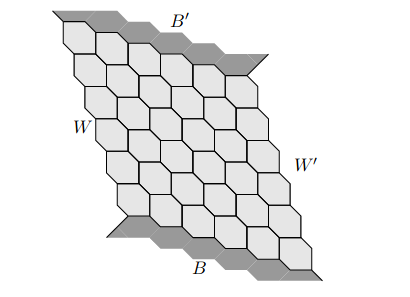
\includegraphics[scale=0.5]{HEX.png}
				
		\subsubsection{Сама теорема}
		
			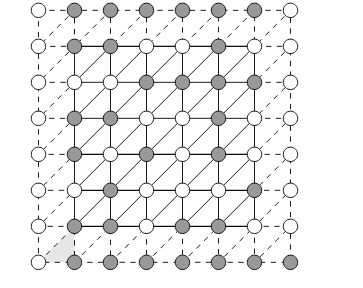
\includegraphics[scale=0.45]{NEWHEX.png}
		
			Теперь заменим гексы на обычную координатную плоскость, причём игра, по сути, останется такой же. Теперь перейдём к самой теореме.
			
			Шар с лёгкостью заменяется на обычный квадрат $[0, 1] \times [0, 1]$
			
			Пусть $f : [0, 1]^2 \rightarrow [0, 1]^2$ ~--- непрерывна. Тогда
			
			$\exists a \in [0, 1]^2$, $f(a) = a$
			
			$a \in [0, 1]^2$
			
			$a = (a_1, a_2)$
			
			$f(x) \in \mathbb{R}^2$
			
			$f(x) = (f(x)_1, f(x)_2)$
			
        \subsubsection{Доказательство}
			
			Пусть $\rho$ ~--- функция, заданная на $[0, 1]^2 \times [0, 1]^2$
				
			$\rho(x, y) = \max \left(|x_1 - y_1|, |x_2 - y_2|\right)$ ~--- непрерывна на $[0, 1]^2$
			
			$x_n \rightarrow a$
				
			$y_n \rightarrow b$
				
			$\rho(x_n, y_n) \rightarrow \rho(a, b)$
				
			Очевидно, что для любых $x, y: x \neq y \Rightarrow \rho(x, y) > 0$
				
		\subsubsection{Теперь к самой теореме}
				
            Пусть для любого $x \in [0, 1]^2$ $f(x) \neq x$. Тогда $\rho(x, f(x)) > 0$, но $\rho$ непрерывно по $x$ и $[0, 1]^2$ ~--- компакт, значит по теореме Вейерштрасса существует такое $\varepsilon > 0$, что
				
			$\min\limits_{x \in [0, 1]^2} \rho(x, f(x)) = \varepsilon > 0$
				
			По теореме Кантора для этого $\varepsilon$ найдётся такая $\delta$ (будем считать, что $\sqrt{2} \delta < \varepsilon$), что
				
			$\forall x, \widehat{x} \in [0, 1]^2 : \| x - \widehat{x} \| < \delta \cdot \sqrt{2} \Rightarrow \| f(x) - f(\widehat{x}) \| < \varepsilon$
				
			Берём $\frac{1}{n} < \varepsilon$
				
			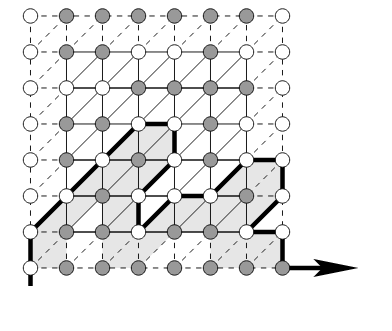
\includegraphics[scale=0.45]{HEXTHEOREM.png}
				
        \subsubsection{Доска}
				
            Узел $(l, k) \rightarrow \left(\frac{l}{n}, \frac{k}{n}\right) \in [0, 1]^2$
				
			$0 \leq l, k \leq n$
				
			Красим узлы
				
			$v$ ~--- логический узел, $v = (v_1, v_2)$
				
			$c(v) = \min \left\{ i : \left\| f\left(\frac{v}{n}\right)_i - \frac{v_i}{n} \right\| \geq \varepsilon \right\}$
			
			По лемме об игре в гексы есть одноцветная тропинка.
				
			Путь $v^0$ ~--- начальная точка тропинки, $v^N$ ~--- конечная.
				
			$v^0_1 = 0$
				
			$f\left(\frac{v^0}{n}\right) \in [0, 1]^2$, т.е. $f\left(\dfrac{v^0}{n}\right)_1 \geq 0$
				
			$\varepsilon \leq f\left(\dfrac{v^0}{n}\right)_1$
				
			Аналогично для $v^N_1 = 1$
				
			$f\left(\frac{v^N}{n}\right)_1 \leq 1$
				
			$f\left(\frac{v^N}{n}\right)_1 - \dfrac{v^N_1}{n} \leq -\varepsilon$
				
			$f\left(\frac{v^0}{n}\right)_1 - \dfrac{v^0_1}{n} \geq \varepsilon$
	
			Поскольку для любых $x$ верно, что $|f(x)_1 - x_1| \geq \varepsilon$, то из этого следует, что какой-то прыжок был длиной не меньше $2 \varepsilon$, но такое невозможно, поскольку по условию если $\| x - \widehat{x} \| < \frac{1}{n}$, то $\| f(x) - f(\widehat{x}) \| < \varepsilon$
				
				
	\newpage

	\section{Теорема о свойствах неопределенного интеграла}
	
		Пусть $f$, $g$ имеют первообразную на $\langle a, b \rangle$. Тогда:
		
		\begin{enumerate}
		
			\item $\int f + \int g  = \int (f + g)$
			
				$\forall \alpha \in \mathbb{R}$ $\int(\alpha f) = \alpha \int{f}$
				
			\item $\forall \varphi: \langle c, d \rangle \rightarrow \langle a, b \rangle$, $\varphi$ дифференцируема
			
				$\int f(\varphi(t))\varphi'(t)dt = F(\varphi(t)) + C$, где $F$ ~--- первообразная $f$
				
			\item $\forall \alpha, \beta \in \mathbb{R}$, $\alpha \neq 0 : \int f(\alpha x + \beta)dx = \frac{1}{\alpha} F(\alpha x + \beta) + C$
			
			\item $f$, $g$ ~--- дифференцируемы на $\langle a, b \rangle$
			
				$f' \cdot g$ имеет первообразную на $\langle a, b \rangle$
				
				Тогда $f \cdot g'$ тоже имеет первообразную и 
				
				$\int f'g = fg - \int fg'$
				
		\end{enumerate}
			
		\textbf{Доказательство}
		
		\begin{enumerate}
		
			\item $(F + G)' = f + g$
			
				$(\alpha F)' = \alpha f$
				
			\item $(F(\varphi(t)))' = f(\varphi(t))\varphi'(t)$
			
			\item $\left(\dfrac{1}{\alpha} F (\alpha x + \beta)\right)' = f(\alpha x + \beta)$
			
			\item $(fg)' = f'g + fg'$, т.е. $fg = \int f'g + \int fg'$
			
		\end{enumerate}
		
	\newpage
	
	\section{Интегрирование неравенств. Теорема о среднем}
	
		\subsection{Интегрирование неравенств}
		
			\subsubsection{Формулировка}
                
                $f$, $g \in C[a, b]$, $f \leq g \Rightarrow \int\limits^b_a f \leq \int\limits^b_a g$
			
            \subsubsection{Доказательство}
            
                Если $0 \leq f \leq g$
			
                $\int\limits^b_a f = \sigma (\PG (f, [a, b])) \leq \sigma (\PG (g, [a, b])) = \int\limits^b_a g$
			
                В общем случае
			
                $\PG(f_+, [a, b]) \subset \PG(g_+, [a, b])$
			
                $\PG(f_-, [a, b]) \supset \PG(g_-, [a, b])$
			
                $\sigma (\PG(f_+, [a, b])) - \sigma (\PG(f_-, [a, b])) \leq \sigma (\PG(g_+, [a, b])) - \sigma (\PG(g_-, [a, b]))$
			
                $\int\limits^b_a f \leq \int^b_a g$
			
			\subsubsection{Следствия}
			
                \begin{enumerate}
                
                    \item $f \in C[a, b]$
                    
                        $\min\limits_{[a, b]} f \cdot (b - a) \leq \int\limits^b_a f \leq \max\limits_{[a, b]} f \cdot (b - a)$
                        
                    \item $f \in C[a, b]$
                    
                        $\left| \int\limits^b_a f \right| \leq \int\limits^b_a \left| f \right|$
                        
                        т.к. $- \int\limits^b_a \left| f \right| \leq \int\limits^b_a f \leq \int\limits^b_a \left| f \right|$
                        
                \end{enumerate}
                
		\subsection{Теорема о среднем значении}
		
			\subsubsection{Формулировка}
			
                Пусть $f$ непрерывна на $[a, b] \Rightarrow \exists c \in [a, b]: \int\limits^b_a f = f(c)(b-a)$
		
            \subsubsection{Доказательство 1 (Кохась порофлил)}
		
                Просто берём прямую и двигаем её сверху вниз, тем самым по теореме о бутерброде мы найдём такое значение $c$, что $\int\limits^b_a f = f(c)(b - a)$
			
            \subsubsection{Нормальное доказательство}
		
                Если $a = b$ ~--- очевидно.
			
                Пусть $a < b$
			
                $\min f \leq \frac{1}{b - a} \int\limits^b_a f \leq \max f$
			
                по теореме Больцано-Коши о промежуточном значении
			
                $\exists c : \frac{1}{b - a} \cdot \int\limits^b_a f = f(c)$
                
                $\int\limits^b_a f = f(c)(b - a)$
			
	\newpage
	
	\section{Теорема Барроу}
	
		\subsection{Определение}
		
			$f \in C[a, b]$, $\varphi : [a, b] \rightarrow \mathbb{R}$
		
			$\varphi (x) = \int\limits^x_a f(t)dt$
		
			Интеграл с верхним переменным пределом
		
		\subsection{Теорема (Барроу)}
		
			В условиях определения оказывается, что $\varphi$ ~--- дифференцируема на $[a, b]$ и $\varphi'(x) = f(x)$ для любого $x \in [a, b]$
		
		\subsection{Доказательство}
		
			Фиксируем $x$ и при $y > x$
		
			$\lim\limits_{y \rightarrow x + 0} \frac{\varphi(y) - \varphi(x)}{y - x} = \lim\limits_{y \rightarrow x + 0} \frac{1}{y - x} \left( \int\limits^y_a f - \int\limits^x_a f \right) = \lim\limits_{y \rightarrow x + 0} \frac{1}{y - x} \int\limits^y_x f = \lim\limits_{y \rightarrow x + 0} f(c) = f(x)$
		
			$\exists c \in [x, y]$ ~--- следует из теоремы о среднем значении.
		
			Аналогично доказываем, что $\lim\limits_{y \rightarrow x - 0} = \ldots = f(c)$
		
		\subsection{Замечания}
		
			\begin{itemize}
			
				\item Интеграл с нижним переменным пределом
				
					$\psi(x) = \int\limits^b_x f$. Тогда $\psi'(x) = -f$
					
				\item Эта теорема также доказывает теорему о существовании неопределенного интеграла.
				
			\end{itemize}
			
	\newpage
	
	\section{Формула Ньютона-Лейбница, в том числе, для кусочно-непрерывных функций}
	
		\subsection{Формулировка теоремы}
		
			Пусть $f$ непрерывна (кусочно-непрерывна) на $[a, b]$, $F$ ~--- (почти) первообразная $f$. 
		
			Тогда $\int\limits^b_a f = F(b) - F(a)$
		
		\subsection{Доказательство}
		
			$\varphi$ (из теоремы Барроу) ~--- тоже первообразная, значит
			
			$\exists c : F = \varphi + c$
			
			$F(b) - F(a) = \Phi(b) - \Phi(a) = \int\limits^b_a f - \int\limits^a_a f = \int\limits^b_a f$
			
			$\int\limits^b_a f = F(b) - F(a)$
			
			При $a > b$ $\int\limits^b_a f \stackrel{\mathrm{def}}{=} - \int\limits^a_b f$
			
        \subsection{Для кусочно-непрерывных функций}
        
            Для кусков функции распишем формулу Ньютона-Лейбница, получим телескопическую сумму, останется только $F(b) - F(a)$
            
	\newpage
	
	\section{Свойства определенного интеграла: линейность, интегрирование по частям, замена переменных}
	
		\subsection{Линейность определенного интеграла}
		
			\subsubsection{Формулировка}
			
                $f, g \in C[a, b]$, $\alpha$, $\beta \in \mathbb{R}$
			
                $\int\limits^b_a \alpha f + \beta g = \alpha \int\limits^b_a f + \beta \int\limits^b_a g$
			
			\subsubsection{Доказательство} 
			
                Из формулы Ньютона-Лейбница
			
                $\int\limits^b_a f = F(b) - F(a) = F(x) \bigg|^b_a$
			
                Для $F$, $G : \alpha F + \beta G$ ~--- первообразная $\alpha f + \beta g$
			
                $\left(\alpha F(x) + \beta G(x)\right) \bigg|^b_a = \alpha F(b) + \beta G(b) - \alpha F(a) - \beta G(a) = \alpha (F(b) - F(a)) + \beta (G(b) - G(a)) = \alpha \int\limits^b_a f + \beta \int\limits^b_a g$
			
		\subsection{Интегрирование по частям}
		
			\subsubsection{Формулировка}
			
                $f, g \in C^{1}[a, b]$. Тогда
			
                $\int\limits^b_a f g' = fg \bigg|^b_a - \int\limits^b_a f'g$
			
			\subsubsection{доказательство}
			
                Из свойств для неопределенного интеграла
			
                $\int\limits^b_a f g' = \left(\int f g'\right) \bigg|^b_a = \left(fg - \int f' g\right) \bigg|^b_a = fg \bigg|^b_a - \int\limits^b_a f'g$
		
		\subsection{Замена переменных}

			\subsubsection{Формулировка}
			
                $f \in C(\langle a, b \rangle)$

                $\varphi : \langle \alpha, \beta \rangle \rightarrow \langle a, b \rangle$

                $\varphi \in C^1 (\langle a, b \rangle)$

                $[p, q] \in \langle \alpha, \beta \rangle$

                Тогда $\int\limits^q_p f(\varphi(t))\varphi'(t) \ dt = \int\limits^{\varphi(q)}_{\varphi(p)} f(x) \ dx$

			\subsubsection{Доказательство}

                Пусть $F$ ~--- первообразная $f$
	
                $F(\varphi(t))$ ~--- первообразная $f(\varphi(t))\varphi'(t)$ на $[p, q]$

                Тогда обе части: $F(\varphi(q)) - F(\varphi(p))$

			\subsubsection{Замечание}

			\begin{enumerate}

				\item Возможен случай $\varphi([p, q]) \supset [\varphi(p), \varphi(q)]$

				\item В другую сторону

					$\int\limits^v_u f(x) \ dx = \int\limits^q_p f(\varphi(t))\varphi'(t) \ dt$

					Тогда подбираем такие $p$ и $q$, что когда $t$ ходит от $p$ до $q$ и $\varphi(t)$ ходит от $v$ до $u$

			\end{enumerate}
	\newpage
	
	\section{Интегральное неравенство Чебышева. Неравенство для сумм}
	
		\subsection{Интегральное неравенство Чебышева}
		
            \subsubsection{Формулировка}
		
                $I_f = \frac{1}{b - a} \int\limits^b_a f$
		
                $f, g \in C[a, b]$ ~--- монотонно возрастают
			
                Тогда $I_f \cdot I_y \leq I_{fg}$
		
                $\int\limits^b_a f \cdot \int\limits^b_a g \leq (b - a) \int\limits^b_a fg$ ~--- неравенство Чебышева
		
            \subsubsection{Доказательство}
		
                $\forall x, y \in [a, b]$ $(f(x) - f(y))(g(x)-g(y)) \geq 0$
			
                Проинтегрируем по переменной $x$ по отрезку $[a, b]$
			
                $f(x)g(x) - f(y)g(x) - f(x)g(y) + f(y)g(y) \geq 0$
			
                $I_{fg} - f(y)I_g - I_f g(y) + f(y)g(y) \geq 0$
			
                Интегрируем по $y$ на $[a, b] : \frac{1}{b - a} \int\limits^b_a$
			
                $I_{fg} - I_f \cdot I_g - I_f \cdot I_g + I_{fg} \geq 0$
			
                $I_{fg} \geq I_f \cdot I_g$
                
        \subsection{Неравенство для сумм}
        
            \subsubsection{Формулировка для сумм}
            
                Пусть задана последовательность $a_n : a_1 \geq a_2 \geq \ldots \geq a_n$ и $b_n : b_1 \geq b_2 \geq \ldots \geq b_n$. Тогда
                
                $\dfrac{1}{n} \sum\limits^n_{k = 1} a_k b_k \geq \left( \dfrac{1}{n} \sum\limits^n_{k = 1} a_k \right) \left( \dfrac{1}{n} \sum\limits^n_{k = 1} b_k \right)$
                
            \subsubsection{Доказательство}
            
                По неравенству Чебышёва
                
                $I_{fg} \geq I_f I_g$
                
                Пусть $I_f = \dfrac{1}{n} \int\limits^n_0 f = \dfrac{1}{n} \sum a_k$
                
                $f(x) = a_{[x + 1]}$, $x \in [0, n]$ (где $[x]$ ~--- округление к ближайшему целому вниз)
                
                $I_g = \dfrac{1}{n} \int\limits^n_0 g = \dfrac{1}{n} \sum b_k$
                
                $g(x) = b_{[x + 1]}$, $x \in [0, n]$
                
                Отсюда следует, что
                
                $\dfrac{1}{n} \sum a_k b_k \geq \left( \dfrac{1}{n} \sum a_k \right) \left( \dfrac{1}{n} \sum b_k \right)$
                
	\newpage
	
	\section{Иррациональность числа $\pi$}
	
		\subsection{Вспомогательный интеграл}
		
			Пусть $H_n = \dfrac{1}{n!} \int\limits^{\dfrac{\pi}{2}}_{-\dfrac{\pi}{2}} \left(\dfrac{\pi^2}{4}-t^2\right)^n \ \cos t \ dt$
			
			$H_n = \begin{bmatrix} f = \left(\dfrac{\pi^2}{4} - t^2\right)^n & g = \sin t \\ f' = -2nt \left(\dfrac{\pi^2}{4} - t^2\right)^{n - 1} & g' = -\cos t \end{bmatrix}$
			
			$H_n = \dfrac{1}{n!} \left(\dfrac{\pi^2}{4} - t^2\right)^n \sin t \bigg|^{\dfrac{\pi}{2}}_{-\dfrac{\pi}{2}} + \dfrac{1}{n!} 2n \int\limits^{\dfrac{\pi}{2}}_{-\dfrac{\pi}{2}} t (\dfrac{\pi^2}{4}-t^2)^{n - 1} \sin t \ dt$
			
			$H_n = \dfrac{1}{n!} 2n \int\limits^{\dfrac{\pi}{2}}_{-\dfrac{\pi}{2}} t (\dfrac{\pi^2}{4}-t^2)^{n - 1} \sin t \ dt$
			
			$H_n = \begin{bmatrix} f = t \left(\dfrac{\pi^2}{4} - t^2\right)^{n - 1} & g = -\cos t \\ f' = \left(\dfrac{\pi^2}{4} - t^2\right)^{n - 1} - 2(n - 1)t^2\left(\dfrac{\pi^2}{4} - t^2\right)^{n - 2} & g' = \sin t \end{bmatrix}$
			
			$f' = \left(\dfrac{\pi^2}{4} - t^2\right)^{n - 1} + 2(n - 1)\left(\dfrac{\pi^2}{4} - t^2\right)^{n - 1} - \dfrac{\pi^2}{2} (n - 1) \left(\dfrac{\pi^2}{4} - t^2\right)^{n - 2}$
			
			$f' = (2n - 1)\left(\dfrac{\pi^2}{4} - t^2\right)^{n - 1} - \dfrac{\pi^2}{2}(n - 1)\left(\dfrac{\pi^2}{4}-t^2\right)^{n - 2}$
			
			$\dfrac{2}{(n - 1)!} t \left(\dfrac{\pi^2}{4} - t^2\right)^{n - 1} (-\cos t) \bigg|^{\dfrac{\pi}{2}}_{-\dfrac{\pi}{2}} - \dfrac{2}{(n - 1)!} \int\limits^{\dfrac{\pi}{2}}_{-\dfrac{\pi}{2}} \left( (2n - 1)\left(\frac{\pi^2}{4} - t^2\right)^{n - 1} - \dfrac{\pi^2}{2} (n - 2) \left(\dfrac{\pi^2}{4} - t^2\right)^{n - 2}\right) \cos t \ dt$
			
			Пусть $n \geq 2$, тогда
			
			$H_n = (4n - 2) H_{n - 1} - \pi^2 H_{n - 2} = \ldots + H_2 + \ldots + H_0$
			
			$H_0 = 2$
			
			$H_1 = 2 \int\limits^{\dfrac{\pi}{2}}_{-\dfrac{\pi}{2}} \dfrac{t}{f} \dfrac{g'}{\sin t} = 2t (- \cos t)\bigg|^{\dfrac{\pi}{2}}_{-\dfrac{\pi}{2}} + 2 \int\limits^{\dfrac{\pi}{2}}_{-\dfrac{\pi}{2}} \cos t \ dt = 4$
			
		\subsection{Теорема}
		
			Число $\pi^2$ ~--- иррациональное (и тогда $\pi$ тоже)
			
		\subsection{Доказательство (от противного)}
		
			Пусть $\dfrac{1}{n!} \int\limits^{\dfrac{\pi}{2}}_{-\dfrac{\pi}{2}} \left(\dfrac{\pi^2}{4} - t^2\right)^n \cos t = P_n (\pi^2)$, где $P_n$ ~--- многочлен с целыми коэффициентами.
			
			$\deg P \leq n$
			
			Этого не может быть
			
			Пусть $\pi^2 = \dfrac{m}{k} \in \mathbb{Q}$. Тогда $k^n P_n\left(\frac{m}{k}\right)$ ~--- целое число
			
			Значит $k^n \cdot P_n \left(\dfrac{m}{k}\right) \geq 1$, т.е.
			
			$\dfrac{k^n}{n!} \int\limits^{\dfrac{\pi}{2}}_{-\dfrac{\pi}{2}} \left(\dfrac{\pi^2}{4} - t^2\right)^n \cos t \ dt \geq 1$
			
			$\dfrac{k^n}{n!} \int\limits^{\dfrac{\pi}{2}}_{-\dfrac{\pi}{2}} \left(\dfrac{\pi^2}{4} - t^2\right)^n \cos t \ dt \leq \dfrac{k^n}{n!} \left(\dfrac{\pi^2}{4}\right)^n \cdot \pi \xrightarrow[n \rightarrow +\infty]{} 0$
			
	\newpage
	
	\newpage

	\section{Формула Тейлора с остатком в интегральной форме}


		\subsection{Формулировка}

			Пусть $\langle a, b \rangle \in \overline{\mathbb{R}}$, $f \in c^{n + 1} (\langle a, b \rangle)$

			$x$, $x_0 \in \langle a, b \rangle$. Тогда

			$f(x) = \sum\limits^n_{k = 0} \frac{f^{(k)} (x_0)}{k!} (x - x_0)^k + \frac{1}{n!} \int\limits^x_{x_0} (x - t)^n f^{(n + 1)}(t) \ dt$

		\subsection{Доказательство (по индукции)}

			\begin{itemize}

				\item $n = 0 : f(x) = f(x_0) = \int\limits^x_{x_0} f'(t) \ dt$

					По формуле Ньютона-Лейбница

				\item Переход от $n$ к $n + 1$

					$f(x) + T_n + \frac{1}{n!} \int\limits^x_{x_0} (x - t)^n f^{(n + 1)} (t) \ dt = \begin{bmatrix} u' (x - t)^n & u = -\frac{(x - t)^{n + 1}}{n + 1} \\ v = f^{n - 1} & v' = f^{(n + 2)} \end{bmatrix}$
						
					$T_n + \frac{1}{n!} \left( -\frac{(x - t)^{n + 1}}{(n + 1)} \cdot f^{(n + 1)} (t) \bigg|^{t = x}_{t = x_0} + \int\limits^x_{x_0} \frac{(x - t)^{n + 1}}{n + 1} \cdot f^{(n + 2)} (t) \ dt \right)$ 
					
					$T_n + \frac{f^{(n + 1)} (x_0)}{(n + 1)!} (x - x_0)^{n + 1} + \frac{1}{(n + 1)!} \int\limits^x_{x_0} (x - t)^{n + 1} f^{(n + 2)} (t) \ dt$

			\end{itemize}

		\subsection{Послесловие}

			$f(x) = \sum\limits^n_{k = 0} \frac{f^{(k)}(x_0)}{k!} (x - x_0)^k + R_n$

			$f(t) = \sum\limits^n_{k = 0} \frac{f^{(k)}(x_0)}{k!} (t - x_0)^k + R_n$

			$F$ ~--- первообразная $f$  $\int\limits^x_{x_0} f(t) \ dt = F(x) - F(x_0)$

			$F(x) - F(x_0) = \sum\limits^n_{k = 0} \int\limits^x_{x_0} \frac{f^{(k)} (x_0)}{k!} (t - x_0)^k \ dt + \int\limits^x_{x_0} R_n = \frac{(t - x_0)^{k + 1}}{k + 1} \bigg|^{t = x}_{t = x_0}$

			$\sum\limits^n_{k = 0} \frac{F^{(k + 1)} (x_0)}{(k + 1)!} (x - x_0)^{k + 1} + \int\limits^x_{x = 0} R_n$

			Мы имеем право формально интегрировать формулу Тейлора

	\newpage

	\section{Лемма об ускоренной сходимости}
	
		\subsection{Формулировка}
		
			Пусть $f$, $g : D \rightarrow \mathbb{R}$, $a$ ~--- предельная точка $D \subset \mathbb{R}$, $a \in \overline{\mathbb{R}}$
		
			Пусть также существует $U(a) : f \neq 0$ и $g \neq 0$ в $\dot{U}(a)$
		
			Пусть $\lim\limits_{x \rightarrow a} f(x) = 0$ и $\lim\limits_{y \rightarrow a} g(x) = 0$ (Также возможен вариант, что $\lim\limits_{x \rightarrow a} f(x) = + \infty$ и $\lim\limits_{y \rightarrow a} g(x) = +\infty$)
			
			Тогда для любой последовательности $x_k \rightarrow a$, $x_k \in D$, $x_k \neq a$ найдётся такая последовательность $y_k \rightarrow a$ ($y_k \in D$, $y_k \neq a$), что 
			
			$\lim\limits_{k \rightarrow +\infty} \frac{f(y_k)}{g(x_k)} = 0$ и $\lim\limits_{k \rightarrow +\infty} \frac{f(y_k)}{f(x_k)} = 0$
			
		\subsection{Доказательство}
		
			\begin{enumerate}
			
				\item Пусть $f$, $g \rightarrow 0$, тогда можно добиться того, что $\left| \frac{f(y_k)}{f(x_k)} \right| < \frac{1}{k}$ и $\left| \frac{f(y_k)}{g(x_k)} \right| < \frac{1}{k}$
			
					Тогда найдётся такое $K$, что $\left| \frac{f(x_k)}{f(x_{2019})} \right| < \frac{1}{2019}$ для любых $k > K \Rightarrow y_{2019} = x_k$
			
					Продолжаем так до бесконечности
			
					$\left| \frac{f(x_i)}{f(x_k)} \right| < \frac{1}{k}$
			
					$\exists i > k$ $\left| \frac{f(x_i)}{f(x_k)} \right| < \frac{1}{k} \Rightarrow y_k := x_i$

					Теперь пусть $\left| \frac{f(x_i)}{g(x_k)} \right| < \frac{1}{k}$ при $x \rightarrow +\infty$ и $\left| \frac{f(x_i)}{g(x_k)} \right| < \frac{1}{k}$ также при $i \rightarrow +\infty$
			
					Тогда для каждого $k$ найдётся такое $K$, что для всех $i > K$ выполняется сразу оба условия, значит присвоим $y_k := x_i$, где $i$ ~--- какое-то число большее $K$.
		
				\item Пусть $f$, $g \rightarrow +\infty$. Считаем, что $f > 0$ и $g > 0$. Пусть $f(x_k)$ и $g(x_k)$ ~--- возрастающие последовательности (остальные случаи рассматриваются аналогично). Тогда
				
					$i = \min n: \begin{cases} f(x_n) \geq \sqrt{g(x_k)} \\ f(x_n) \geq \sqrt{f(x_k)} \end{cases}$
					
					Возьмём $y_k := x_{i - 1}$
					
					Тогда $\frac{f(y_k)}{f(x_k)} < \frac{\sqrt{f(x_k)}}{f(x_k)} = \frac{1}{\sqrt{f(x_k)}} \rightarrow 0$
					
						$\frac{f(y_k)}{g(x_k)} < \frac{\sqrt{g(x_k)}}{g(x_k)}= \frac{1}{\sqrt{g(x_k)}} \rightarrow 0$
					
			\end{enumerate}	
			
	\newpage
	
	\section{Правило Лопиталя (с леммой)}
	
		\subsection{Формулировка}
			
			Пусть $f$, $g$ ~--- дифференцируемы на $(a, b \rangle$, $g' \neq 0$ на $(a, b \rangle$ и существует $\lim\limits_{x \rightarrow a} \frac{f'(x)}{g'(x)} = A \in \overline{\mathbb{R}}$
			
			Не стоит забывать, что $\lim\limits_{x \rightarrow a + 0} \dfrac{f(x)}{g(x)}$ ~--- неопределенно.
			
			Тогда $\lim\limits_{x \rightarrow a} \frac{f(x)}{g(x)} = A$
			
		\subsection{Пример из жизни}
		
			Пусть $f$, $g : [0, +\infty) \rightarrow \mathbb{R}$
			
			Пусть $f$ ~--- сколько прошёл студент, 	
			
				$g$ ~--- сколько прошёл Кохась.
				
			Тогда $f$, $g \rightarrow +\infty$, но если сравним скорости $f'$ и $g'$, то легко узнать, на сколько больше прошёл Кохась, чем студент.
			
		\subsection{Доказательство}
		
			$g' \neq 0 \Rightarrow g'$ сохраняет знак (по теореме Дарбу), значит $g$ ~--- строго монотонна
			
			\begin{enumerate}
			
				\item $g \rightarrow +\infty \Rightarrow g > 0$ в окрестности точки $a$
				
				\item $g \rightarrow 0$,
					
					$g \uparrow \ \Rightarrow g > 0$ в окрестности точки $a$
			
					$g \downarrow \ \Rightarrow g < 0$ в окрестности точки $a$
					
			\end{enumerate}
			
		\subsection{Собственное доказательство}
		
			Берём последовательность $y_k \rightarrow a$ из леммы.
			
			По теореме Коши $\exists \xi_k \in [x_k, y_k]$ (не факт, что $x_k \leq y_k$)
			
			$\frac{f(x_k) - f(y_k)}{g(x_k) - g(y_k)} = \frac{f'(\xi_k)}{g'(\xi_k)}$
			
			Домножаем правую и левую часть на $\dfrac{g(x_k) - g(y_k)}{g(x_k)}$
			
			$\frac{f(x_k)}{g(x_k)} = \frac{f(y_k)}{g(x_k)} + \frac{f'(\xi_k)}{g'(\xi_k)} \left( 1 - \frac{g(y_k)}{g(x_k)} \right)$
			
			$\frac{f(x_k)}{g(x_k)} \rightarrow \frac{f'(\xi_k)}{g'(\xi_k)}$
			
	\newpage
	
	\section{Теорема Штольца}
	
		\subsection{Формулировка}
		
			Пусть $x_n$, $y_n \rightarrow 0$
			
			$\lim\limits_{n \rightarrow +\infty} \frac{x_n}{y_n} = \left[ \frac{0}{0} \right]$
			
			Тогда если существует $\lim\limits_{n \rightarrow +\infty} \frac{x_n - x_{n - 1}}{y_n - y_{n - 1}} = a \in [0, +\infty]$
			
			Также $y_n$ ~--- строго монотонна (если $a = 0$, то $x_n$ ~--- тоже строго монотонна)
			
			Тогда $\exists \lim\limits_{n \rightarrow +\infty} \frac{x_n}{y_n} = a$
			
		\subsection{Доказательство}
		
			\begin{enumerate}
			
				\item Пусть $a > 0$, $a$ ~-- конечное, тогда можно считать, что $y_n \geq y_{n - 1}$ из монотонности и $x_n \geq x_{n - 1}$ при больших $n$.
			
					Заметим обидный факт, что $\frac{a}{b} \cdot \frac{c}{d} = \frac{ac}{bd}$ и $\frac{a}{b} : \frac{c}{d} = \frac{a : c}{b : d}$, но $\frac{a}{b} + \frac{c}{d} \neq \frac{a + c}{b + d}$. Кохасю обидно, поэтому будем считать, что $\frac{a}{b} + \frac{c}{d} = \frac{a + c}{b + d}$. Если вы с этим не согласны, то окей, но заметим, что справедливо:
			
					$0 < \alpha < \frac{a}{b} < \beta$
			
					$0 < \alpha < \frac{c}{d} < \beta$
			
					$\alpha < \frac{a + c}{b + d} < \beta$
			
					Вернёмся к самой теореме
			
					$\forall \varepsilon > 0$ $(\varepsilon < a)$ $\exists N_1$ $\forall n > N \geq N_1$
			
					$a - \varepsilon < \frac{x_{N + 1} - x_N}{y_{N + 1} - y_N} < a + \varepsilon$
			
					$a - \varepsilon < \frac{x_{N + 2} - x_{N + 1}}{y_{N + 2} - y_{N + 1}} < a + \varepsilon$
			
					$\vdots$
			
					$a - \varepsilon < \frac{x_n - x_{n - 1}}{y_n - y_{n - 1}} < a + \varepsilon$
			
					Складываем всё
			
					$a - \varepsilon < \frac{x_n - x_N}{y_n - y_N} < a + \varepsilon$
			
					Устремляем $n$ к $+\infty$
			
					$a - \varepsilon \leq \frac{x_N}{y_N} < a + \varepsilon$
			
				\item Если $a = +\infty$ ~--- аналогично
				
					$\forall E > 0$ $\exists N_1$, $\forall n > N \geq N_1$ $\frac{x_{N + 1} - x_{N}}{y_{N + 1} - y_N} > E$
					
					$E < \frac{x_n - X_N}{y_n - y_N}$
					
					$E \leq \frac{x_N}{y_N}$
					
				\item Если $a = 0$, то $\lim\limits_{n \rightarrow +\infty} \frac{y_n}{x_n} = +\infty$
				
				\item Если $a < 0$ ~--- меняем знаки
				
			\end{enumerate}						
		
	\newpage
	
	\section{Пример неаналитической функции}
	
		\subsection{Неалитическая функция}
		
			$f(x) = \begin{cases} e^{-\frac{1}{x^2}}, & x \neq 0 \\ 0, & x = 0 \end{cases}$
			
		\subsection{Утверждение}
		
			$f$ ~--- бесконечное дифференцируема на $\mathbb{R}$
			
			($\forall x \in \mathbb{R} \ \ \ \forall k \in \mathbb{N} \ \ \ \exists f^{(k)} (x)$)
			
		\subsection{Доказательство}
		
			Если $x \neq 0$ ~--- то очевидно
			
			Пусть $x = 0$, тогда для любого $k$ $\exists f^{(k)} (0) = 0$
			
			Из теоремы Лагранжа:
			
			Если $\exists \lim\limits_{x \rightarrow a + 0} f'(x) = \lim\limits_{x \rightarrow a - 0} f'(x) = L$, где $L \in \mathbb{R}$, то
			
			$f$ ~--- дифференцируема и $f'(a) = L$
			
			$f'(x) = \dfrac{2}{x^3} \cdot e^{\left(-\dfrac{1}{x^2}\right)}$, $x \neq 0$
			
			$\lim\limits_{x \rightarrow 0} \dfrac{\dfrac{1}{x^3}}{e^{\left(\dfrac{1}{x^2}\right)}} = \left[ \dfrac{\infty}{\infty} \right] = \lim\limits_{x \rightarrow 0} \dfrac{-\dfrac{3}{x^4}}{-\dfrac{2}{x^3} e^{\left(\dfrac{1}{x^2}\right)}} = \lim\limits_{x \rightarrow 0} \dfrac{3}{2} \cdot \dfrac{\dfrac{1}{x}}{e^{\left(\dfrac{1}{x^2}\right)}} = \lim\limits_{x \rightarrow 0} \dfrac{-\dfrac{1}{x^2}}{-\dfrac{2}{x^3} e^{\left(\dfrac{1}{x^2}\right)}} = \lim\limits_{x \rightarrow 0} \cdot x \cdot e^{\left(-\dfrac{1}{x^2}\right)} \rightarrow 0$
			
			$\lim\limits_{x \rightarrow 0} \dfrac{1}{x^k} \cdot e^{\left(-\dfrac{1}{x^2}\right)} = \left(\lim\limits_{x \rightarrow 0} \dfrac{\dfrac{1}{x^2}}{e^{\left(\dfrac{1}{x^2} \cdot \dfrac{2}{k}\right)}} \right)^{\dfrac{k}{2}} = \left( \lim\limits_{x \rightarrow 0} \dfrac{-\dfrac{1}{x^3}}{-\dfrac{4}{k} \cdot \dfrac{1}{x^3} \cdot e^{\left(\dfrac{1}{x^3}\right)}} \right)^{\dfrac{k}{2}} = 0$
			
			\underline{Итого}
			
			$f'(x) = \dfrac{2}{x^3} \cdot e^{\left(-\dfrac{1}{x^2}\right)}$, $x \neq 0$
			
			$f'(0) = 0$
			
			Аналогично
			
			$f'' = -\dfrac{6}{x^4} \cdot e^{\left(-\dfrac{1}{x^2}\right)} - \dfrac{4}{x^5} \cdot e^{\left(-\dfrac{1}{x^2}\right)}$, $x \neq 0$
			
			$\lim\limits_{x \rightarrow 0} f''(x) = 0 \Rightarrow f''(0) = 0$
			
			$x \neq 0$ $f^{(k)} (x) = P_k \left(\dfrac{1}{x}\right) \cdot e^{\left(-\dfrac{1}{x^2}\right)}$
			
			$\lim\limits_{x \rightarrow 0} f^{(k)}(x) = 0 \Rightarrow f^{(k)}(0) = 0$
			
	\newpage

	\section{Интеграл как предел интегральных сумм}

		\subsection{Формулировка}

			Пусть $f \in C[a, b]$

			Тогда $\forall \varepsilon > 0 \ \exists \delta > 0$ что для любого дробления $\mathcal{T} \ a = x_0 < x_1 < \ldots < x_n = b$ ранга меньше $\delta$ и любого оснащения $\xi_1, \xi_2, \ldots, \xi_n$

			$\left| \sum\limits^n_{k = 1} f(\xi_k)(x_k - x_{k - 1}) - \int\limits^b_a f(x) \ dx \right| < \varepsilon$

		\subsection{Доказательство}

		\begin{enumerate}
			\item Поделим на отрезки в соответствии с дроблением. Очевидно, что $\int\limits^b_a = \sum\limits^n_{k = 1} \int\limits^{x_k}_{x_{k - 1}}$. Тогда рассмотрим разность

				$\int\limits^{x_k}_{x_{k - 1}} f(\xi_k) \ dx - \int\limits^{x_k}_{x_{k - 1}} f(x) \ dx$

				$\int\limits^{x_k}_{x_{k - 1}} (f(\xi_k) - f(x) \ dx) \rightarrow 0$, т.к. $x_{k - 1} \rightarrow x_k$, а $\xi_k \in [x_{k - 1}, x_k]$

			\item По теореме Кантора о равномерной непрерывности

				$\forall \varepsilon > 0 \ \exists \delta > 0 \ \forall x_1, x_2: \left| x_1 - x_2 \right| < \delta \ \left| f(x_1) - f(x_2) \right| < \frac{\varepsilon}{b - a}$ <<Китайский $\varepsilon$>>

				Берём $x_0, x_1, \ldots, x_n, \xi_1, \xi_2, \ldots, \xi_n$

				$\left| \sum\limits^n_{k = 1} - \int\limits^b_a \right| = \left| \sum\limits^n_{k = 1} \int\limits^{x_k}_{x_{k - 1}} f(\xi_k) \ dx - \sum\limits^n_{k = 1} f(x) \ dx \right| = \left| \sum\limits^n_{k = 1} \int\limits^{x_k}_{x_{k - 1}} \left( f(\xi_k) - f(x) \right) \ dx \right| \leq \sum\limits^n_{k = 1} \int\limits^{x_k}_{x_{k - 1}} \left| f(\xi_k) - f(x) \right| \ dx$

				$\left| \xi_k - x_k \right| < \delta$ для любых $[x_{k - 1}, x_k]$ (по условию)

				$\leq \sum\limits^n_{k = 1} \int\limits^{x_k}_{x_{k - 1}} \frac{\varepsilon}{b - a} \ dx = \int\limits^b_a \frac{\varepsilon}{b - a} \ dx = \varepsilon$

		\end{enumerate}

		\subsection{Замечания}

			\begin{enumerate}

				\item $\int\limits^b_a f(x) \ dx = \lim\limits_{\lambda (\mathcal{T}) \rightarrow 0} \sum\limits^n_{k = 1} f(\xi_k)(x_k - x_{k - 1})$

				\item $\omega(\delta) := \sup\limits_{x, t \\ \left| x - t \right| < \delta} \left| f(x) - f(t) \right|$ ~--- модуль непрерывной функции $f$

					По теореме Кантора $f$ ~--- непрерывна $\Longrightarrow \omega(\delta) \xrightarrow[f \rightarrow 0]{} 0$
					
					$\omega(\delta)$ монотонно убывает на отрезке

					$\sum\limits^n_{k = 1} \int\limits^{x_k}_{x_{k - 1}} \left| f(\xi_k) - f(x) \right| \ dx \leq \sum \int \omega(\delta) \ dx = \omega(\delta) (b - a)$

					Пусть $f$ ~--- дифференцируема на $[a, b] \ \left| f' \right| \leq M$

					$\left| f(x) - f(t) \right| \leq M \left| x - t \right|$ ~--- следствие из теоремы Лагранжа

					$\left| f(\xi_k) - f(x) \right| \leq M \delta \left| \xi_k - x \right|$

					$\left| \sum - \int \right| \leq M \delta (b - a)$
				
			\end{enumerate}

	\newpage

	\section{Теорема об интегральных суммах для центральных прямоугольников}

		\subsection{Формулировка}

			Пусть $f \in C^2[a, b] \ a = x_0 < x_1 < \ldots < x_n = b$

			$\delta := \max \left| x_k - x_{k - 1} \right|$

			Тогда 

			$\left| \sum\limits^n_{i = 1} f \left( \frac{x_i + x_{i - 1}}{2} \right) (x_i - x_{i - 1}) - \int\limits^b_a f(x) \ dx \right| \leq \frac{\delta^2}{8} \cdot \int\limits^b_a |f''|$

		\subsection{Доказательство}

			$\int\limits^{x_i}_{x_{i - 1}} f(x) \ dx = \int\limits^{\xi_i}_{x_{i - 1}} + \int\limits^{x_i}_{\xi_i} = \begin{bmatrix} u = f & u' = f' \\ v' = 1 & v = x - x_{i - 1} \end{bmatrix}$ и $\begin{bmatrix} u = f & u' = f' \\ v' = 1 & v = x - x_i \end{bmatrix}$ 
				
			$f(x)(x - x_{i - 1}) \bigg|^{x = \xi_i}_{x = x_{i - 1}} - \int\limits^{\xi_i}_{x_{i - 1}} f'(x)(x - x_{i - 1}) \ dx + f(x)(x - x_i) \bigg|^{x = x_i}_{x = \xi_i} - \int\limits^{x_i}_{\xi_i} f'(x)(x - x_i) \ dx = f(\xi_i)(\xi_i - x_{i - 1}) + f(\xi_i)(x_i - \xi_i) - \left( f'(x) \frac{(x - x_{c - 1})^2}{2} \bigg|^{x = \xi_i}_{x = x_{i - 1}} - \int\limits^{\xi_i}_{x_{i -1 }} f''(x) \frac{(x - x_{i - 1})^2}{2} \ dx + f'(x) \frac{(x - x_i)^2}{2} \bigg|^{x_i}_{\xi_i} - \int\limits^{x_i}_{\xi_i} f''(x) \frac{(x - x_i)^2}{2} \right) = f(\xi_i)(x_i - x_{i - 1}) + \int\limits^{x_i}_{x_{i - 1}} f''(x) \ \varphi(x) \ dx$

			$Пусть \varphi(x) = \begin{cases} \frac{(x - x_{i - 1})^2}{2}, \ x \in [x_{i - 1}, \xi_i] \\ \frac{(x - x_i)^2}{2}, x \in [\xi_i, x_i] \end{cases}$
			
			Тогда $\varphi(x)$ определена на $[a, b]$

			$\left| \sum\limits^n_{i = 1} f \left( \frac{x_{i - 1} - x_i}{2} \right) (x_i - x_{i - 1}) - \int\limits^b_a f(x) \ dx \right| = \left| \sum\limits^n_{i = 1} \left( f(x_i)(x_i - x_{i - 1}) - \int\limits^{x_i}_{x_{i - 1}} f \right) \right| = \left| \sum \left( - \int\limits^{x_i}_{x_{i - 1}} f''(x) \varphi(x) \ dx \right) \right| = \left| \int\limits^b_a f''(x) \varphi(x) \ dx \right| \leq \int\limits^b_a | f''(x) | \varphi(x) \ dx \leq \frac{\delta^2}{8} \int\limits^b_a | f'' |$

			Поскольку $\max \varphi(x) = \frac{(\frac{\delta}{2})^2}{2} = \frac{\delta^2}{8}$

	\newpage

	\section{Теорема о формуле трапеций, формула Эйлера--Маклорена}

		\subsection{Формулировка теоремы о формуле трапеций}

			Пусть $f \in C^2[a, b] \ a = x_0 < x_1 < \ldots < x_n = b \ \ \ \delta = \max (x_i - x_{i - 1})$

			Тогда $\left| \sum\limits^n_{i = 1} \frac{f(x_{i - 1}) + f(x_i)}{2} (x_i - x_{i - 1}) - \int\limits^b_a f(x) \ dx \right| \leq \frac{\delta^2}{8} \int\limits^b_a |f''|$

		\subsection{Доказательство}

			$\int\limits^{x_i}_{x_{i - 1}} f(x) = \begin{bmatrix} u = f & u' = f' \\ v'1 = 1 & v = x - \xi_i \end{bmatrix}$ 
			
			$f(x)(x - \xi_i) \bigg|^{x_i}_{x_{i - 1}} - \int\limits^{x_i}_{x_{i - 1}} f'(x)(x - \xi_i) - f(x_{i - 1})(x_{i - 1} - \xi_i) - \left(f'(x) \bigg|^{x_i}_{x_{i - 1}} - \int\limits^{x_i}_{x_{i - 1}} f'' \frac{(x - \xi_i)^2}{2} \ dx \right) = \left(f(x_i) + f(x_{i - 1}) \right) \frac{x_i - x_{i - 1}}{2} - \left( f'(x) - \frac{1}{2} \psi(x) \bigg|^{x_i}_{x_{i - 1}} - \int\limits^{x_i}_{x_{i - 1}} f'' (-\frac{1}{2} \psi(x)) \ dx \right)$

			$\begin{bmatrix} u = f' & u' = f'' \\ v' = (x - \xi_i) & \psi(x) = (x - x_{i - 1})(x_i - x) \end{bmatrix} \ x \in [x_{i - 1}, x_i]$ на $[a, b]$

			$v = -\frac{1}{2} \psi(x)$

			$(f(x_i) + f(x_{i - 1}) \cdot \frac{(x_i - x_{i - 1})}{2} - \frac{1}{2} \int\limits^{x_i}_{x_{i - 1}} f'' \psi(x) \ dx$

			$\left| \sum\limits^n_{i = 1} \frac{f(x_{i - 1}) + f(x_i)}{2} \cdot (x_i - x_{i - 1}) - \int\limits^b_a f(x) \ dx \right| = \left| \sum\limits^n_{i = 1} \left( \frac{f(x_{i - 1}) + f(x_i)}{2}(x_i - x_{i - 1}) - \int\limits^{x_i}_{x_{i - 1}} f(x) \ dx \right) \right| = \left| \sum\limits^n_{i = 1} \frac{1}{2} \int\limits^{x_i}_{x_{i - 1}} f''(x) \psi(x) \ dx \right| = \frac{1}{2} \int\limits^b_a \left| f''(x) \right| \psi(x) \ dx \leq \frac{\delta^2}{8} \int\limits^b_a \left| f'' \right|$

		\subsection{Простейший случай формулы Эйлера-Маклорена}

			$m, n \in \mathbb{Z} \ f \in C^2[m, n]$. Тогда

			$\int\limits^n_m f(x) \ dx = (\sum\limits^n_{i = m})^{\triangledown} f(i) - \frac{1}{2} \int\limits^n_m f''(x) \left\{ x \right\} (1 - \left\{ x \right\}) \ dx$

			Очевидно$^{TM}$, что это формула трапеции.

			$[a, b] \leftrightarrow [m, n] \ x_0 = m, x_1 = m + 1, \ldots, x_{last} = n$

			$\left\{ x \right\} (1 - \left\{ x \right\})$ ~--- парабола между двумя целыми точками
		
    \newpage
    
    \section{Асимптотика степенных сумм}
        
        $f(x) = x^p$
        
        $1^p + 2^p + \ldots + n^p = \int\limits^n_1 x^p dx + \dfrac{n^p + 1}{2} + \dfrac{1}{2} \int\limits^n_1 (x^p)'' \left\{ x \right\} (1 - \left\{ x \right\}) dx$
            
        $1^p + 2^p + \ldots + n^p = \dfrac{n^{p + 1}}{p + 1} - \dfrac{1^{p + 1}}{p + 1} + \dfrac{n^p}{2} + \dfrac{1}{2} + \dfrac{p(p - 1)}{2} \int\limits^n_1 x^{p - 2} \left\{ x \right\} (1 - \left\{ x \right\})$
            
        $1^p + 2^p + \ldots + n^p = \dfrac{n^{p + 1}}{p + 1} + \dfrac{n^p}{2} + O(\max(1, n^{p - 1}))$
    
    \newpage
    
    \section{Асимптотика частичных сумм гармонического ряда}
    
        $1 + \dfrac{1}{2} + \ldots + \dfrac{1}{n} = \int\limits^n_1 \dfrac{1}{x} dx + \dfrac{1}{2} + \dfrac{1}{2n} + \int\limits^n_1 \dfrac{1}{x^3} \left\{ x \right\}(1 - \left\{ x \right\}) dx$
        
        $1 + \dfrac{1}{2} + \ldots + \dfrac{1}{n} = \ln n + \dfrac{1}{2} + \dfrac{1}{2n} + \int\limits^n_1 \dfrac{\left\{ x \right\}(1 - \left\{ x \right\})}{x^3} dx$
        
        Интеграл постоянной возрастает и ограничен сверху $\dfrac{1}{4} \int\limits^n_1 \dfrac{1}{x^3} dx = -\dfrac{1}{x^2} \cdot \dfrac{1}{8} \bigg|^{x = n}_{x = 1} < \dfrac{1}{8}$
        
        Всё, что правее логарифма ~--- постоянная Эйлера или $\gamma$
        
        Итого
        
        $1 + \dfrac{1}{2} + \ldots + \dfrac{1}{n} = \ln {n} + \gamma + o(1)$
        
    \newpage
    
    \section{Формула Валлиса}
    
        \subsection{Формулировка}
        
            $\lim\limits_{n \rightarrow \infty} \left( \dfrac{(2n)!!}{(2n - 1)!!} \right)^2 \cdot \dfrac{1}{2n} = \dfrac{\pi}{2}$
            
        \subsection{Доказательство}
        
            $I_n = \int\limits^{\dfrac{\pi}{2}}_0 \sin^n x dx = \begin{bmatrix} u = sin^{n - 1} x & u' = (n - 1) \sin^{n - 2} x cos x \\ v' = \sin {x} dx & v = -\cos{x} \end{bmatrix}$
            
            $-\cos{x} \sin^{n - 1} x \bigg|^{\dfrac{\pi}{2}}_0 + (n - 1) \int\limits^{\dfrac{\pi}{2}}_0 \sin^{n - 2} x \cos^2 x dx = (n - 1) \int\limits^{\dfrac{\pi}{2}}_0 (\sin^{n - 2} x - sin^n x) dx = (n - 1) (I_{n - 2} - I_n)$
            
            $I_n = \dfrac{n - 1}{n} I_{n - 2}$
            
            $I_0 = \int\limits^{\dfrac{\pi}{2}}_0 1 dx = \dfrac{\pi}{2}$
            
            $I_1 = \int\limits^{\dfrac{\pi}{2}}_0 \sin x dx = -\cos{x} \bigg|^{\dfrac{\pi}{2}}_0 = 1$
            
            $I_n = \dfrac{n - 1}{n} I_{n - 2} = \dfrac{n - 1}{n} \cdot \dfrac{n - 3}{n - 4} I_{n - 4} = \ldots$
            
            Посчитаем отдельно для случая чётного и нечётного $n$
            
            $I_{2n + 1} = \dfrac{2n}{2n + 1} \cdot {2n - 2}{2n - 1} \cdot \ldots \cdot 1 = \dfrac{(2n)!!}{(2n + 1)!!}$
            
            $I_{2n} = \dfrac{2n - 1}{2n} \cdot {2n - 3}{2n - 2} \cdot \dfrac{\pi}{2} = \dfrac{(2n - 1)!!}{(2n)!!} \cdot \dfrac{\pi}{2}$
            
            Так как при $x \in \left[ 0, \dfrac{\pi}{2} \right] \ \ \ \sin^{2k + 1} x \leq \sin^{2k}$
            
            То и $I_{n + 1} \leq I_n$
            
            Также, $I_{2n + 1} \leq I_{2n} \leq I_{2n - 1}$
            
            $\dfrac{(2n)!!}{(2n + 1)!!} \leq \dfrac{\pi}{2} \dfrac{(2n - 1)!!}{(2n)!!} \leq \dfrac{(2n - 2)!!}{(2n - 1)!!}$
            
            Разность правой и левой части стремится к $0$, значит 
            
            $\exists \lim\limits_{k \rightarrow +\infty} \dfrac{1}{2k} \left( \dfrac{(2k)!!}{(2k - 1)!!} \right)^2 = \dfrac{\pi}{2}$
            
    \newpage
    
    \section{Формула Стирлинга}
    
        \subsection{Формулировка}
        
            $n! \sim n^n e^{-n} \sqrt{2 \pi n}$ при $n \rightarrow +\infty$
            
        \subsection{Доказательство}
        
            $\sqrt{\pi} = \dfrac{1}{\sqrt{k}} \dfrac{(2k)!!}{(2k - 1)!!} = \lim\limits_{k \rightarrow +\infty} \dfrac{2 \cdot 4 \cdot 6 \cdot \ldots \cdot (2k)}{1 \cdot 3 \cdot \ldots \cdot (2k - 1)} \cdot \dfrac{1}{\sqrt{k}}$
            
            $\sqrt{\pi} = \lim \dfrac{(2 \cdot 4 \cdot \ldots \cdot (2k))^2}{(2k)!} \cdot \dfrac{1}{\sqrt{k}} = \lim \dfrac{2^{2k} (k!)^n}{(2k)!} \cdot \dfrac{1}{\sqrt{k}}$
            
            $\sqrt{\pi} = \lim\limits_{k \rightarrow \infty} \dfrac{2^{2k} (k^k \cdot e^{-k} \sqrt{k} \cdot c)^2}{\sqrt{k} (2k)^{2k} e^{-2k} \sqrt{2k} \cdot c} = \lim\limits_{k \rightarrow \infty} \dfrac{2^{2k} \cdot k^{2k} \cdot e^{-2k} \cdot k \cdot c^2}{\sqrt{2} \cdot k \cdot 2^{2k} \cdot k^{2k} \cdot e^{-2k} \cdot c} = \dfrac{c}{\sqrt{2}}$
            
            $c = \sqrt{2 \pi}$
            
    \newpage
    
    \section{Теорема о вычислении аддитивной функции промежутка по плотности}
    
        \subsection{Формулировка}
        
            Пусть заданы $f$ и $\phi$ на $\langle a, b \rangle$, $f$ ~--- непрерывна, $\phi$ ~--- аддитивная функция промежутка, $f$ ~--- плотность $\phi$
            
            Тогда $\forall [p, q] \subset \langle a, b \rangle \ \phi([p, q]) = \int\limits^q_p f(x) \ dx$
            
        \subsection{Доказательство}
        
            Можно принять за факт, что у нас дан промежуток $[a, b]$ (если это не так, то уменьшим его чуть-чуть и переобозначим)
            
            $F(x) = \begin{cases} 0{,} & x = a \\ \phi([a, x]){,} & x > a \end{cases}$ ~--- первообразная $f$
            
            $\inf\limits_{[x, x + h]} f \leq \frac{\phi([x, x + h])}{h} \leq \sup\limits_{[x, x + h]} f$
            
            $x : F'_+(x) = \lim\limits_{h \rightarrow 0 + 0} \frac{F(x + h) - F(x)}{h} = \lim \frac{\phi([a, x + h]) - \phi([a, x])}{h} = \lim \frac{\phi([x, x + h])}{h} = \lim\limits_{h \rightarrow 0 + 0} f(x + \Theta h) = f(x)$, где
            
            $0 \leq \Theta \leq 1$
            
            $\Theta = \Theta(h)$
            
            Аналогично посчитаем и $F'_-(x)$
            
            $\phi([p, q]) = F(q) - F(p) = \int\limits^q_p f(x) \ dx$
            
    \newpage
    
    \section{Обобщенная теорема о плотности}
    
        \subsection{Формулировка}
            
            Пусть $f : \langle a, b \rangle \rightarrow \mathbb{R}$ ~--- непрерывная функция, $\phi : \Segm \langle a, b \rangle \rightarrow \mathbb{R}$ ~--- аддитивная функция.
        
            Пусть $\forall \Delta \subset \Segm \langle a, b \rangle$ заданы числа $m_{\Delta}$, $M_{\Delta}$.
        
            \begin{enumerate}
        
                \item $m_{\Delta} \cdot l(\Delta) \leq \phi(\Delta) \leq M_{\Delta} \cdot l(\Delta)$
            
                \item $\forall x \in \Delta$ $m_{\Delta} \leq f(x) \leq M_{\Delta}$
            
                \item $\forall x \in \langle a, b \rangle$ $M_{\Delta} - m_{\Delta} \rightarrow 0$, если $l(\Delta) \rightarrow 0$, $x \in \Delta$
            
            \end{enumerate}
        
            $\forall \varepsilon > 0 \ \ \ \exists \delta > 0 \ \ \ \forall \Delta \in \Segm \ \ \ \langle a, b \rangle : x \in \Delta, \ \ \ l(\Delta) < \delta$
            
            $\left| M_{\Delta} - m_{\Delta} \right| < \varepsilon$
        
            Тогда $f$ ~--- плотность $\phi$ (и $\forall [p, q]$ $\phi([p, q]) = \int\limits^q_p f(x) \ dx$)
        
        \subsection{Доказательство}
        
            $F(x) = \begin{cases} 0, & x = 0 \\ \phi([a, x]), & x > a \end{cases}$
        
            Дифференцируем $F_+$
        
            $m_{\Delta} \leq \frac{F(x+ h) - F(x)}{h} \leq M_{\Delta}$
        
            $\left| \frac{F(x + h) - F(x)}{n} - f(x) \right| \leq \left| M_{\Delta} - m_{\Delta} \right| \xrightarrow[h \rightarrow 0]{} 0$, $\Delta = [x, x + h]$
        
            $\frac{F(x + h) - F(x)}{h} \xrightarrow[h \rightarrow 0]{} f(x)$
        
            Аналогично и с $F_-$
        
    \newpage
    
    \section{Площадь криволинейного сектора: в полярных координатах и для параметрической кривой}
    
        \subsection{Введение}
        
            Площадь подграфика $f : \langle a, b \rangle \rightarrow \mathbb{R}$ ~--- непрерывная, $f \geq 0$
        
            $\phi([p, q]) = \sigma \PG (f, [p, q])$ ~--- аддитивная функция. Мы знаем, что $\phi([p, q]) = \int\limits^q_p f(x) \ dx$, $f$ ~--- плотность

        \subsection{Пример}
        
            $\frac{x^2}{a^2} + \frac{y^2}{b^2} = 1$
            
            $\sigma$(эллипса) $ = 2 \sigma(\PG(b \sqrt{1 - \frac{x^2}{a^2}}{,} [-a, a])) =  2 \cdot \int\limits^a_{-a} b \sqrt{1 - \frac{x^2}{a^2}} dx$
            
            Путь $\gamma : [\alpha, \beta] \rightarrow \mathbb{R}^2$, $x = a \cos t$
            
            $[0, 2 \pi] \longmapsto (a \cos t, b \sin t)$
            
            $2 \int\limits^0_{\pi} b \sqrt{1 - \cos^2 t} / a(-\sin t) \ dt = 2 a b \int\limits^0_{\pi} - \sin^2 t \ dt = 2 a b \int\limits^{\pi}_{0} \sin^2 t \ dt = 2 a b \int\limits^{\pi}_{0} \frac{1 - \cos {2t}}{2} \ dt = \pi a b$
            
        \subsection{Теорема}
            
            $[\alpha, \beta] \subset [0, 2 \pi)$
            
            $\rho : [\alpha, \beta] \rightarrow \mathbb{R}$ ~--- непрерывная, $\rho \geq 0$
            
            $A = \left\{ (r, \phi) : \phi \in [\alpha, \beta] \ 0 \leq r \leq \rho(\phi) \right\}$ ~--- <<Аналог ПГ>>
            
            Тогда $\sigma(A) = \frac{1}{2} \int\limits^{\beta}_{\alpha} \rho^2(\phi) \ d \phi$
            
        \subsection{Доказательство}
        
            $[\alpha, \beta] \longmapsto \sigma(A)$ ~--- функция промежутка $Segm [\alpha, \beta]$ ~--- аддитивная функция.
            
            Проверим, что $\frac{1}{2} \rho^2 (\phi)$ ~--- плотность
            
            $[\gamma, \delta]$ ~--- строим $A_{\gamma{,} \delta}$
            
            $\sigma (A_{\gamma{,} \delta}) \leq \sigma$(Круговой сектор $(0, \max\limits_{[\gamma, \delta]} \rho(\phi), [\gamma, \delta])$)
            
            $\sigma (A_{\gamma{,} \delta}) \geq \sigma$(Круговой сектор $(0, \min\limits_{[\gamma, \delta]} \rho(\phi), [\gamma, \delta])$)
            
            $\min\limits_{[\gamma, \delta]} \frac{1}{2} \rho(\phi) l([\gamma, \delta]) \leq \sigma (A_{\gamma{,} \delta}) \leq \max\limits_{[\gamma, \delta]} \frac{1}{2} \rho(\phi) l([\gamma, \delta])$
            
            По определению плотности
            
        \subsection{Замечание}
        
            $(x(t), y(t))$ $t \in [a, b]$
            
            $x = r \cos \phi$
            
            $y = r \sin \phi$
            
            $r = \sqrt{x^2 + y^2}$
            
            $\phi = \arctg \frac{y}{x}$
            
            $\begin{cases} r(t) = x(t)^2 + y(t)^2 \\ \phi = \arctg \frac{y}{x} \end{cases}$ ~--- параметрическое задание того же пути в полярных координатах
            
            $\sigma A = \frac{1}{2} \int\limits^{\phi_1}_{\phi_0} r^2 (\phi) \ d \phi = \frac{1}{2} \int\limits^{t_1}_{t_0} (x(t)^2 + y(t)^2) (\arctg \frac{y(t)}{x(t)} ) \ dx = \frac{1}{2} \int\limits^{t_1}_{t_0} (x^2 + y^2) \frac{1}{1 + \frac{y^2}{x^2}} - \frac{y'x - x'y}{x^2} \ dt = \frac{1}{2} \int\limits^{t_1}_{t_0}(y'(t)x(t) - x'(t)y(t))$
            
            $\phi = \arctg \frac{y(t)}{x(t)}$
            
            Площадь круга
            
            $x = \cos t$
            
            $y = \sin t$
            
            $S = \frac{1}{2} \int\limits^{2\pi}_0 \cos^2 t - (-\sin t) \sin t \ dt = \frac{1}{2} \int\limits^{2\pi}_0 1 = \frac{2\pi}{2} = \pi$
            
            $x = \cos t$
            
            $y = -\sin t$
            
            $S = \frac{1}{2} \int\limits^{2\pi}_0 -\cos^2 t - \sin^2 t \ dt = - \pi$
            
            Она ловит ориентированную площадь
            
            $x = x(t) = a \cos t$
            
            $y = y(t) = b \sin t$
            
            $\sigma = \int\limits^b_a y(x) \ dx = \int\limits^b_a y \ dx$
            
            $\sigma$(эллипса) = $\int\limits^a_{-a} y(x) \ dx = \int\limits^a_{-a} y \ dx = \int\limits^0_{\pi} y(t) x'(t) dy$
            
            $x = x(t)$
            
    \newpage
    
    \section{Изопериметрическое неравенство}
    
        \subsection{Формулировка}
        
            Пусть $G$ ~--- замкнутая выпуклая фигура в $\mathbb{R}^2$
            
            $\diam G < 1$ ($\diam G = \sup\limits_{x, y \in G} \rho(x, y)$)
            
            Тогда $\sigma(G) \leq \frac{\pi}{4}$
            
        \subsection{Доказательство}
        
            $f(x) = \sum \left\{ t : [(x, 0), (x, t)] \cap G = \varnothing \right\}$
            
            $g(x)$ ~--- аналогично
            
            $f(x)$ ~--- выпуклая
            
            $\phi \in \left[ -\frac{\pi}{2}, \frac{\pi}{2} \right]$
            
            $r(-\frac{\pi}{2}) = r(\frac{\pi}{2}) = 0$
            
            $r(\phi)$ ~--- непрерывная функция от $\phi$
            
            $\sigma(G) = \frac{1}{2} \int\limits^{\frac{\pi}{2}}_{-\frac{\pi}{2}} r^2 (\phi) \ d \phi = \frac{1}{2} \left( \int\limits^0_{-\frac{\pi}{2}} + \int\limits^{\frac{\pi}{2}}_0 \right)$
            
            $\frac{1}{2} \int\limits^{\frac{\pi}{2}}_0 r^2 (\phi - \frac{\pi}{2}) + r^2 (\phi) \ d \phi = \frac{1}{2} \int\limits^{\frac{\pi}{2}}_0 AB^2 \ d \phi \leq \frac{1}{2} \int\limits^{\frac{\pi}{2}}_0 1 \ d \phi = \frac{\pi}{4}$
            
    \newpage
    
    \section{Вычисление длины гладкого пути}
    
        \subsection{Формулировка}
        
            Пусть $\gamma : [a, b] \rightarrow \mathbb{R}^m$, $\gamma \in C^1$.
            
            Тогда $l(\gamma) = \int\limits^b_a \| \gamma'(t) \| dt$
            
        \subsection{Доказательство}
        
            Будем дополнительно считать, что $\gamma' \neq 0$
            
            $\gamma$ ~--- инъективно. Если это не так, то разобьём на несколько частей, и каждую из них посчитаем отдельно.
            
            $\phi : Segm[a, b] \rightarrow \mathbb{R}$
            
            $[p, q] \rightarrow l\left(\gamma|_{[p, q]} \right)$
            
            Пусть $\phi$ ~--- аддитивная функция промежутка по аксиоме 2. Проверим, что $\| \gamma'(t) \|$ ~--- её плотность
            
            Это значит, что $\forall \Delta : \exists m_{\Delta}, M_{\Delta}$ и выполняются следующие свойства:
            
            \begin{enumerate}
            
                \item $l(\Delta) m_{\Delta} \leq \phi(\Delta) \leq M_{\Delta} l(\Delta)$
                
                \item $m_{\Delta} \leq f(x) \leq M_{\Delta}$, $x \in \Delta$
                
                \item $\Delta \rightarrow x$ $M_{\Delta} - m_{\Delta} \rightarrow 0$
                
            \end{enumerate}
            
            $\Delta \supset [a, b]$, $\gamma(t) = (\gamma_1(t), \gamma_2(t), \ldots, \gamma_m(t))$
            
            $m_i(\Delta) = \min\limits_{t \in \Delta} | \gamma'_i(t) |$
            
            $M_i(\Delta) = \max\limits_{\Delta} |\gamma'_i(t) |$
            
            $m_{\Delta} = \sqrt{\sum m_i(\Delta)^2}$
            
            $M_{\Delta} = \sqrt{\sum M_i{\Delta}^2}$
            
            Очевидно, что при любом $t \in \Delta$ $m_{\Delta} \leq \| \gamma'(t) \|  \leq M_{\Delta}$, где $\| \gamma'(t) \| = \sqrt{\sum(\gamma'_i(t))^2}$
            
            При $\Delta \rightarrow x$ $M_{\Delta} - m_{\Delta} \rightarrow 0$ по непрерывности $\gamma'_i(t)$ в точке $t = x$.
            
            Проверим, что $m_{\Delta} l(\Delta) \leq \phi(\Delta) \leq M_{\Delta} l(\Delta)$
            
            $\widetilde{\gamma} : \Delta \rightarrow \mathbb{R}^m$ $\widetilde{\gamma}(t) = \left(M_1(\Delta)t, M_2(\Delta)t, \ldots, M_m(\Delta)t\right) = M \cdot t$, где $M = (M_1(\Delta), M_2(\Delta), \ldots, M_m(\Delta) )$
            
            Отображение $T : C_{\gamma} \rightarrow C_{\overline{\gamma}}$ $\gamma(t) \mapsto \overline{\gamma}(t)$ ~--- проверим, что расстяжение
            
            $\rho(\gamma(t_0), \gamma(t_1)) = \sqrt{\sum\limits_{i = 1}^n (\gamma_i(t_0) - \gamma_i(t_1))^2} = \sqrt{\sum(\gamma'_i(\mathcal{T}_i))^2(t_0 - t_1)^2} \leq \sqrt{\sum M_i{\Delta}^2 |t_0 - t_1|} = \rho(T(\gamma(t_0)), T(\gamma(t_1)))$, значит $T$ ~--- растяжение
            
            $l\left( \gamma|_{\Delta} \right) \leq l(\widetilde{\gamma})$, т.е. $\phi(\Delta) \leq M_{\Delta} l(\Delta)$.
            
            Аналогично $\phi(\Delta) \geq m_{\Delta}l(\Delta)$ ~--- сжатие.
            
            Значит $\| \gamma' \|$ ~--- плотность
            
    \newpage
    
    \section{Объем фигур вращения}
    
        \subsection{Формулировка}
            Обозначим фигуры, полученную вращением по оси $x$ за $T_x(A) = \left\{ (x, y, z) : (x, \sqrt{y^2 + z^2}) \in A \right\}$
        
            По оси $y$ ~--- $T_y(A) = \left\{ (x, y, z) : (\sqrt{x^2 + z^2}, y^2) \in A \right\}$
        
            Пусть $f \in C[a, b]$, $f \geq 0$
            
            Тогда:
            
            \begin{enumerate}
            
                \item $V(T_x(\PG(f, [a, b]))) = \pi \int\limits^b_a f^2(x) \ dx$
                
                \item $[a, b] \subset [0, +\infty) \ V(T_y(\PG(f, [a, b]))) = 2 \pi \int\limits^b_a x f(x) \ dx$
                
            \end{enumerate}
            
        \subsection{Доказательство}
        
            $\phi: \Delta \in Segm([a, b]) \mapsto V(T_{x \ or \ y} (\PG(f, \Delta)))$ ~--- аддитивная функция.
            
            $\pi \min\limits_{x \in \Delta} f(x) \cdot l(\Delta) = V(F_{\Delta}) \leq \phi(\Delta) \leq V(\varepsilon_{\Delta}) = \pi \max\limits_{x \in \Delta} f(x) \cdot l(\Delta)$
            
            $\varepsilon_{\Delta}$ ~--- цилиндр прямой круговой
            
            $\varepsilon_{\Delta} = T_x(\PG(\max\limits_{\Delta} f, \Delta)) = \Delta B(0, \max\limits_{\Delta} f) \in \mathbb{R}^3$
            
            $\mathbb{R} \times \mathbb{R}^2$
            
            $\phi(\Delta)$ ~--- плотность, $\pi \int\limits^b_a f^2(x) dx$
            
            $\Delta : m_{\Delta}, M_{\Delta}$
            
            \begin{enumerate}
            
                \item $m_{\Delta} l(\Delta) \leq \phi(\Delta) \leq M_{\Delta} l(\Delta)$
                
                \item $m_{\Delta} \leq f(x) \leq M_{\Delta}$, $x \in \Delta$
                
                \item $\Delta \rightarrow x$ $M_{\Delta} - m_{\Delta} \rightarrow 0$
                
            \end{enumerate}
            
            $V(T_y(\PG(f, [a, b]))) = 2 \pi \int\limits^b_a x \cdot f(x) dx$
            
            $F_{\Delta} = T_y(\PG(\min\limits_{\Delta} f, \Delta))$
            
            $\phi(\Delta) \leq V(\varepsilon_{\Delta}) = \sigma(ring) \cdot \max\limits_{\Delta} f = \pi(q^2 - p^2) \cdot \max\limits_{[p, q]} f = \pi (p + q) \max f(p - q) \leq \pi \cdot \max\limits_{x \in [p, q]} (2x) \cdot \min\limits_{x \in [p, q]} f(x) \cdot (q - p)$
            
            Аналогично
            
            $\pi \min\limits_{x \in [p, q]} \cdot \min\limits_{x \in [p, q]} f(x) (q - p)$
            
            \begin{enumerate}
            
                \item $m_{\Delta} l(\Delta) \leq \phi(\Delta) \leq M_{\Delta} l(\Delta)$
                
                    $\phi(\Delta) = \pi \cdot 2 x \cdot f(x) \leq \pi \max (2x) \cdot max f(x)$
                    
                \item $m_{\Delta} \leq f(x) \leq M_{\Delta}$
                
                \item $p \rightarrow x_0$, $q \rightarrow x_0$ $\pi \cdot 2 x_0 \cdot f(x_0)$
                
            \end{enumerate}
        
    \newpage
    
    \section{Неравенство Йенсена для сумм}
    
        \subsection{Формулировка}
        
            Пусть $f$ ~--- выпукла на $\langle a, b \rangle$. Тогда
            
            $\forall x_1, x_2, \ldots, x_n \in \langle a, b \rangle$
            
            $\forall \alpha_1, \alpha_2, \ldots, \alpha_n \geq 0$, $\sum\limits_{i = 1}^n \alpha_i = 1$
            
            $f(\alpha_1 x_1 + \alpha_2 x_2 + \ldots + \alpha_n x_n) \leq \alpha_1 f(x_1) + \alpha_2 f(x_2) + \ldots + \alpha_n f(x_n)$
            
        \subsection{Доказательство}
        
            Если все $x$ совпадают, то тривиально.
            
            Пусть $x^* = \alpha_1 x_1 + \alpha_2 x_2 + \ldots + \alpha_n x_n$
            
            $x_{\min} \sum\limits_{i = 1}^n \alpha_i \leq x^* \leq x_{\max} \sum\limits_{i = 1}^n \alpha_i$
            
            $a \leq x_{\min} \leq x^* \leq x_{\max} \leq b$
            
            К любой выпуклой функции можно провести опорную прямую $y = l(x) : f(x) \geq l(x)$, при $x = x_0$ $f(x_0) = l(x_0)$
            
            Проведём к $x^*$ опорную прямую $l(x) = kx + b$
            
            $f(x^*) = l(x^*) = k \sum \alpha_i  x_i + b = \sum\limits_{i = 1}^n k \alpha_i x_i + \sum\limits_{i = 1}^n b \alpha_i = \sum \alpha_i (k x_i + b) = \sum \alpha_i l(x_i) \leq \sum \alpha_i f(x_i)$
            
    \newpage
    
    \section{Неравенство Йенсена для интегралов}
    
        \subsection{Формулировка}
        
            Пусть $f$ ~--- выпукла и непрерывна на $\langle A, B \rangle$
            
            $\varphi : [a, b] \rightarrow \langle A, B \rangle$ ~--- непрерывна
            
            $\lambda : [a, b] \rightarrow [0, +\infty]$, $\int\limits^b_a \lambda = 1$ ~--- непрерывна
            
            Тогда $f\left( \int\limits^b_a \lambda(x) \varphi(x) dx \right) \leq \int\limits^b_a \lambda(x) f(\varphi(x)) dx$
        \subsection{Доказательство}
        
            $m := \inf \varphi(x)$
            
            $M := \sup \varphi(x)$
            
            $c := \int\limits^b_a \lambda(x) \varphi(x) dx \leq \int\limits^b_a \lambda(x) dx \cdot M = M \leq b$
            
            $c \geq m = a$ ~--- аналогично, значит $c \in \langle a, b \rangle$
            
            Если $m = M$ ~--- тривиально
            
            Пусть $y = kx + b$ ~--- опорная прямая к графику $f$ в точке $c$
            
            $f(C) = kC + b = k \int\limits^b_a \lambda \varphi + b \int\limits^b_a \lambda = \int\limits^b_a \lambda(k\varphi + b) \leq \int\limits^b_a \lambda (f \circ \varphi)$
            
            $f\left( \int\limits^b_a \lambda \varphi \right) \leq \int\limits^b_a \lambda (f \circ \varphi)$
            
    \newpage
    
    \section{Неравенство Коши (для сумм и для интегралов)}
    
        \subsection{Неравенство для сумм}
        
            \subsubsection{Формулировка}
            
                Пусть $a_1, a_2, \ldots, a_n > 0$
                
                Тогда $\dfrac{a_1 + a_2 + \ldots + a_n}{n} \geq \sqrt[n]{a_1 a_2 \ldots a_n}$
                
            \subsubsection{Доказательство}
            
                $\ln(\frac{1}{n} a_1 + \frac{1}{n} a_2 + \ldots + \frac{1}{n} a_n) \geq? \frac{1}{n} \ln(a_1 a_2 \ldots a_n) = \frac{1}{n} \ln{a_1} + \frac{1}{n} \ln{a_2} + \ldots + \frac{1}{n} \ln{a_n}$
                
                $x_1 = a_1$
                
                $x_2 = a_2$
                
                $\ldots$
                
                $x_n = a_n$
                
                $\alpha_1 = \alpha_2 = \ldots = \alpha_n = \frac{1}{n}$
                
                $f(\sum \alpha_i x_i) \geq \sum \alpha f(x_i)$, поскольку функция $\ln$ ~--- вогнута
                
        \subsection{Неравенство для интегралов}
        
            \subsubsection{Формулировка}
                $\frac{1}{b - a} \int\limits^b_a f$ ~--- среднее арифметическое $f$ на $[a, b]$
            
                $\exp\left(\frac{1}{b - a} \int\limits^b_a \ln f \right)$ ~--- среднее геометрическое функции $f$ ($f > 0$)
            
                Тогда если $f \in C[a, b \rangle$, $f > 0$
                
                $\exp\left(\frac{1}{b - a} \int\limits^b_a \ln f \right) \leq \frac{1}{b - a} \int\limits^b_a f$
                
                $\frac{1}{b - a} \int\limits^b_a \ln f \leq \ln \left( \frac{1}{b - a} \int\limits^b_a f \right)$
                
                $\ln \longleftrightarrow f$ ~--- вогнутая
                
                $f \longleftrightarrow \varphi$
                
                $\frac{1}{b - a} \longleftrightarrow \lambda$
                
    \newpage
    
    \section{Неравенство Гёльдера для сумм}
    
        \subsection{Формулировка}
        
            Пусть $p > 1$, $\frac{1}{p} + \frac{1}{q} = 1$
            
            $q = \frac{p}{p - 1}$
            
            $a_i, b_i > 0$ для всех $i = 1..n$
            
            Тогда $\sum\limits^n_{i = 1} a_i b_i \leq (\sum a_i^p)^{\frac{1}{p}} (\sum b_i^q)^{\frac{1}{q}}$
            
            Если $(a_1^p, a_2^p, \ldots, a_n^p) \parallel (b_1^q, b_2^q, \ldots, b_n^q)$ ~--- равенство
            
        \subsection{Доказательство}
            
            $x^p$ ~--- строго выпукла при $p > 1$ и $x > 0$
            
            $(x^p)'' = p(p - 1)x^{p - 2} > 0$
            
            По неравенству Йенсена $\sum\limits_{i = 1}^n \alpha_i x_i)^p \leq \sum\limits_{i = 1}^n \alpha_i x_i^p$
            
            $\alpha_i := \dfrac{b_i^q}{\sum b_i^q}$
            
            $\alpha_i > 0$, $\sum \alpha_i = 1$
            
            Выберем такие $x_i$, что
            
            $\alpha_i \cdot x_i = a_i \cdot b_i$
            
            $x_i = \dfrac{a_i b_i}{\alpha_i} = \dfrac{a_i b_i}{b_i^q} \sum\limits_{j = 1}^n b_j^q = a_i b_i^{1 - q} \sum\limits_{j = 1}^n b_j^q = a_i b_i^{1 - \frac{p}{p - 1}} \sum\limits_{j = 1}^n b_j^q = a_i b_i^{\frac{p - 1 - p}{p - 1}} \sum\limits_{j = 1}^n b_j^q = a_i \cdot b_i^{-\frac{1}{p - 1}} \sum\limits_{j = 1}^n b_j^q$
            
            Тогда $\alpha_i x_i = a_i b_i$
            
            $(\sum\limits_{i = 1}^n \alpha_i x_i)^p = (\sum\limits_{i = 1}^n a_i b_i)^p$
            
            Тогда $\alpha_i x_i^p = a_i^p(\sum\limits_{j = 1}^n b_i^q)^{p - 1}$
            
            Тогда $\sum\limits_{i = 1}^n \alpha_i x_i^p = (\sum\limits_{i = 1}^n a_i^p)(\sum\limits_{j = 1}^n b_j^q)^{p - 1} = (\sum\limits_{i = 1}^n a_i^p)(\sum\limits_{j = 1}^n b_j^q)^{\frac{p}{q}}$
            
            Тогда $(\sum_{i = 1}^n a_i b_i)^p \leq (\sum\limits_{i = 1}^n a_i^p)(\sum\limits_{j = 1}^n b_j^q)^{\frac{p}{q}}$
            
            Возведём в степень $\frac{1}{p}$ и получим исходное неравенство
            
    \newpage
    
    \section{Неравенство Гёльдера для интегралов}
    
        \subsection{Формулировка}
        
            Пусть $\frac{1}{p} + \frac{1}{q} = 1$, $p > 1$
            
            Пусть также $f$, $g \in C[a, b]$ и $f, g \geq 0$ на $[a, b]$. Тогда
            
            $\int\limits^b_a fg \leq \left(\int\limits^b_a f^p\right)^{\frac{1}{p}} \left(\int\limits^b_a g^q\right)^{\frac{1}{q}}$
            
        \subsection{Доказательство}
        
            Делим $[a, b]$ на $n$ равных частей
            
            $x_k = a + k \cdot \frac{b - a}{n}$  $\Delta x_k = x_k - x_{k - 1} = \frac{b - a}{n}$
            
            $\xi_k := x_k$
            
            $a_k := |f(x_k)|(\Delta x_k)^{\frac{1}{p}}$
            
            $b_k := |g(x_k)|(\Delta x_k)^{\frac{1}{q}}$
            
            $a_k \cdot b_k = |f(x_k)g(x_k)| \cdot \Delta x_k$
            
            $\sum\limits_{k = 1}^n |f(x_k) g(x_k)| \Delta x_k \leq (\sum |f(x_k)|^p \Delta x_k)^{\frac{1}{p}}(\sum|g(x_k)|^q \Delta x_k)^{\frac{1}{q}}$
            
            Из неравенства Гёльдера для сумм
            
            $\int\limits^b_a |f(x) g(x)| dx \leq (\int\limits^b_a |f|^p)^{\frac{1}{p}}(\int\limits^b_a |g|^q)^{\frac{1}{q}}$
            
    \newpage
    
    \section{Неравенство Минковского}
    
        \subsection{Формулировка}
        
            Пусть $p \geq 1$
            
            Тогда $\left( \sum\limits_{i = 1}^n |a_i + b_i|^p\right)^{\frac{1}{p}} \leq \left( \sum |a_i|^p \right)^{\frac{1}{p}} + \left( \sum |b_i|^p \right)^{\frac{1}{p}}$
            
            $a_i, b_i \in \mathbb{R}$
            
        \subsection{Замечания}
        
            \begin{itemize}
            
                \item Здесь нет буквы $q$
                
                \item Неравенство Минковского означает, что $(a_1, a_2, \ldots, a_n) \mapsto \left( \sum |a_i|^p \right)^{\frac{1}{p}}$ является нормой
                
            \end{itemize}

        \subsection{Доказательство}
        
            При $p = 1$ ~--- очевидно
            
            $p > 1$ ~--- применим Гёльдера
            
            Пусть $a_i, b_i > 0$
            
            $\sum |a_i| |a_i + b_i|^{p - 1} \leq \left( \sum |a_i|^p \right)^{\frac{1}{p}} \left( \sum |a_i + b_i|^p \right)^{\frac{1}{q}}$
            
            $\sum |b_i| |a_i + b_i|^{p - 1} \leq \left( \sum |b_i|^p \right)^{\frac{1}{p}} \left( \sum |a_i + b_i|^p \right)^{\frac{1}{q}}$
            
            $\sum |a_i + b_i|^p \leq \sum ( |a_i| + |b_i| ) |a_i + b_i|^p \leq \left( \sum |a_i|^p \right)^{\frac{1}{p}} + \left( \sum |b_i|^p \right)^{\frac{1}{p}} (\sum |a_i + b_i|^p)^{\frac{1}{q}}$
            
            $\left( \sum |a_i + b_i|^p \right)^{\frac{1}{p}} \leq \ldots \leq \left( \sum |a_i|^p \right)^{\frac{1}{p}} \left( \sum |b_i|^p \right)^{\frac{1}{p}}$
            
    \newpage
    
    \section{Свойства верхнего и нижнего пределов}
    
        \subsection{Формулировка}
        
            Пусть $x_n$, $x_n'$ ~--- произвольные последовательности. Тогда
            
            \begin{enumerate}
            
                \item $\varliminf x_n \leq \varlimsup x_n$
                
                \item $\forall n \ \ \ x_n \leq x_n'$. Тогда
                
                    $\varlimsup x_n \leq \varlimsup x_n'$
                    
                    $\varliminf x_n \leq \varliminf x_n'$
                    
                \item $\forall \lambda > 0$
                
                    $\varlimsup(\lambda x_n) = \lambda \cdot \varlimsup x_n$
                    
                    $\varliminf(\lambda x_n) = \lambda \cdot \varliminf x_n$
                    
                \item $\varlimsup (-x_n) = -\varliminf(x_n)$
                
                    $\varliminf (-x_n) = -\varlimsup(x_n)$
                    
                \item $\varlimsup (x_n + x_n') \leq \varlimsup x_n + \varlimsup x_n'$
                    
                    $\varliminf (x_n + x_n') \geq \varliminf x_n + \varliminf x_n'$
                    
                    Если правые части имеют смысл
                    
                \item $t_n \rightarrow l \in \overline{\mathbb{R}}$ 
                
                    $\varlimsup (x_n + t_n) = \varlimsup x_n + \lim t_n$
                
                    Если правая часть имеет смысл
                    
                \item $t_n \rightarrow l > 0, l \in \mathbb{R}$ 
                
                    $\varlimsup(x_n \cdot t_n) = l \cdot \varlimsup x_n$
                
            \end{enumerate}
            
        \subsection{Доказательство}
        
            \begin{enumerate}
            
                \item Следует из того факта, что $z_n \leq x_n \leq y_n$
                
                \item $y_n \leq y'_n$
                
                \item $\sup(\lambda A) = \lambda \sum(a)$
                
                \item $\sup(-A) = -\inf(A)$
                
                \item $\sum(x_n + x_n', x_{n + 1} + x_{n + 1};, \ldots) \leq y_n + y_n'$, т.к. это верхняя граница для всех сумм над $\sup$
                
                \item $l \in \mathbb{R}$, тогда $\forall \varepsilon > 0 \exists N_0: \forall k > N_0$
                
                    $x_k + l - \varepsilon < x_k + t_k < x_k + l_k + \varepsilon$
                    
                    $y_n + l - \varepsilon \leq \sum(x_n + t_n, x_{n + 1} + t_{n + 1}, ldots) \leq y_n + l + \varepsilon$, при $N \rightarrow +\infty$
                    
                    $(\varlimsup x_n) + l - \varepsilon \leq \varlimsup (x_n + y_n) \leq (\varlimsup x_n) + l + \varepsilon$
                    
                \item Без доказательства
                
            \end{enumerate}
            
    \newpage
    
    \section{Техническое описание верхнего предела}
    
        \subsection{Формулировка}
        
            \begin{enumerate}
            
                \item $\varlimsup x_n = +\infty \Longleftrightarrow x_n$ ~--- не ограничена сверху
                
                \item $\varlimsup x_n = -\infty \Longleftrightarrow x_n \rightarrow -\infty$
                
                \item $\varlimsup x_n = l \in \mathbb{R} \Longrightarrow$:
                
                \begin{itemize}
                
                    \item $\forall \varepsilon > 0 : \exists N: \forall n > N \ \ \ x_n < l + \varepsilon$
                    
                    \item $\forall \varepsilon > 0$ неравенство $x_n > l - \varepsilon$ выполняется для бесконечного множества номеров $n$
                
                \end{itemize}
                
            \end{enumerate}
            
        \subsection{Доказательство}
        
            \begin{enumerate}
            
                \item Очевидно, что $x_n < y_n$, $y_n$ убывает Таким образом, если $\lim y_n = +\infty \Longrightarrow y_n = +\infty \Longleftrightarrow x_n$ ~--- не ограничена сверху
                
                \item $y_n \rightarrow -\infty$, $\forall E : \exists N : \forall n > N \ x_n \leq y_n < E \Rightarrow \forall E > 0 : \exists N : \forall n > N : x_n < E$, $\forall n > N : y_n \leq E$
                
                \item $x_n \leq y_n$, $y_n \rightarrow l$
                
                \begin{itemize}
                
                    \item $\Rightarrow)$ $\forall \varepsilon > 0 : \exists N : \forall n > N x_n \leq y_n < l + \varepsilon$
                    
                        Если $\exists N_0 : \forall N_0 \forall n < l - \varepsilon$, то $\forall n > N_0 y_n = \sup(\ldots) \leq l - \varepsilon$ и тогда $y_n \rightarrow l$
                        
                    \item $\Leftarrow)$ $\forall \varepsilon : \exists N : \forall n > N y_n \leq l + \varepsilon$, $y_n$ ~--- супремум
                    
                        $x_k \geq l - \varepsilon \Rightarrow y_n \geq l - \varepsilon \Rightarrow y_n \rightarrow l$
                        
                \end{itemize}
                
            \end{enumerate}
            
    \newpage
    
    \section{Теорема о существовании предела в терминах верхнего и нижнего пределов}
    
        \subsection{Формулировка}
        
            Пусть существует $\lim x_n = l \in \overline{\mathbb{R}}$, тогда и только тогда $\varlimsup x_n = \varliminf x_n = l$
            
        \subsection{Доказательство}
        
            \begin{itemize}
            
                \item $\Rightarrow)$ $\lim x_n = +\infty \Longleftrightarrow \varliminf x_n = +\infty \Rightarrow \varliminf \leq \varlimsup x_n = +\infty$
                
                    $\lim x_n = -\infty \Longleftrightarrow \varliminf x_n \leq \varlimsup = -\infty$
                    
                    $\lim x_n \in \mathbb{R}$ ~--- очевидно
                    
                \item $\Leftarrow)$ $z_n \leq x_n \leq y_n$, то по теореме о сжатой последовательности $x_n \rightarrow l$, поскольку $z_n \rightarrow l$ и $y_n \rightarrow l$
                
            \end{itemize}
        
    \newpage
    
    \section{Теорема о характеризации верхнего предела как частичного}
    
        \subsection{Формулировка}
            
            \begin{enumerate}
            
                \item Пусть $l$ ~--- частный предел $x_n$, тогда $\varliminf x_n \leq l \leq \varlimsup x_n$
                
                \item Существуют такие $n_k$, $m_k$, что $\lim x_{n_k} = \varlimsup x_n$ и $\lim x_{m_k} = \varliminf x_n$
                
            \end{enumerate}
            
        \subsection{Доказательство}
        
            \begin{enumerate}
            
                \item Пусть $x_{n_j} \rightarrow l$
                
                    $z_{n_j} \leq x_{n_j} \leq y_{n_j}$, где $z_{n_j} \rightarrow \varliminf x_n$, $x_{n_j} \rightarrow l$, $y_{n_j} \rightarrow \varlimsup x_n$
                    
                \item $\varlimsup x_k = \pm \infty$ ~--- очевидно
                
                    $\varlimsup x_k = l \in \mathbb{R}$ ~--- очевидно
                    
                    Для $\varepsilon = \frac{1}{k}$ $\exists x_{n_k} : l - \frac{1}{k} \leq x_{n_k} \leq l + \frac{1}{k}$
                    
            \end{enumerate}
            
    \newpage
    
    \section{Простейшие свойства несобственного интеграла}
    
        \subsection{Формулировка}
        
            \begin{enumerate}
            
                \item Критерий Больцано-Коши сходимости несобственного интеграла
                
                    Сходимость интеграла $\int\limits^{\rightarrow b}_a f$ равносильна 
                    
                    $\forall \varepsilon > 0 : \exists \Delta \in (a, b) : \forall B_1, B_2 : \Delta < B_1 < B_2 < b : \left| \int\limits^{B_2}_{B_1} f \right| < \varepsilon$
                    
                \item $f$ ~--- допустима на $[a, b]$ и $C \in (a, b)$. Тогда
                
                    $\int\limits^{\rightarrow b}_a f$ и $\int\limits^{\rightarrow b}_c f$ сходятся и расходятся одновременно, и при этом в случае сходимости $\int\limits^{\rightarrow b}_a = \int\limits^c_a + \int\limits^{\rightarrow b}_c$
                    
                \item Пусть $f$, $g$ ~--- допустимы на $[a, b)$, а также
                
                    $\int\limits^{\rightarrow b}_a f$ и $\int\limits^{\rightarrow b}_a g$ сходятся. Пусть $\lambda \in \mathbb{R}$, тогда
                    
                    $\lambda f$ и $f \pm g$ ~--- допустимые функции и
                    
                    $\int\limits^{\rightarrow b}_a \lambda f = \lambda \int\limits^{\rightarrow b}_a f$ и $\int\limits^{\rightarrow b}_a f \pm g = \int\limits^{\rightarrow b}_a f \pm \int\limits^{\rightarrow b}_a g$
                    
                \item Пусть $\int\limits^{\rightarrow b}_a f$ и $\int\limits^{\rightarrow b}_a g$ существуют в $\overline{\mathbb{R}}$, $f \leq g$ на $[a, b)$ Тогда
                
                    $\int\limits^{\rightarrow b}_a f \leq \int\limits^{\rightarrow b}_a g$
                    
                \item Пусть $f$, $g$ ~--- дифференцируемы на $[a, b)$, $f'$, $g'$ ~--- допустимы на $[a, b)$. Тогда (при существовании двух из трёх пределов)
                
                    $\int\limits^{\rightarrow b}_a f g' = fg \bigg|^{\rightarrow b}_a - \int\limits^{\rightarrow b}_a f'g$
                    
                \item Пусть $\varphi : [\alpha, \beta) \rightarrow \langle A, B \rangle$, $\varphi \in C^1$, $f \in C \left( \langle A, B \rangle \right)$. Пусть также существует $\varphi(\beta - 0) \in \overline{\mathbb{R}}$. Тогда
                
                    $\int\limits^{\rightarrow b}_a (f \circ \varphi) \cdot \varphi' = \int\limits^{\varphi(\beta - 0)}_{\varphi(\alpha)} f$
                    
            \end{enumerate}
        
        \subsection{Доказательство}
        
            \begin{enumerate}
            
                \item Положим $\Phi(A) = \int\limits^A_a f$. Сходимость интеграла равносильна сходимости $\Phi(A)$ при $A \rightarrow b - 0$. Воспользуемся критерием Больцано-Коши, а также учтём, что $\Phi(B) - \Phi(A) = \int\limits^B_a$
                
                $$\forall \varepsilon > 0 : \exists \Delta \in (a, b) : \forall B_1, B_2 : \Delta < B_1 < B_2 < b : \left| \Phi(B_2) - \Phi(B_1) \right| < \varepsilon$$
                
                \item При всех $A \in (c, b)$ согласно аддитивности интеграла
                
                    $$\int\limits^A_a f = \int\limits^c_a f + \int\limits^A_c f$$
                    
                \item Аналогично предыдущему пункту возьмём такие $A$ и согласно линейности интеграла
                
                    $$\int\limits^A_a (\alpha f + \beta g) = \alpha \int\limits^A_a f + \beta \int\limits^A_a g$$
                    
                \item Также выберем $A$ и очевидно, что
                
                    $$\int\limits^A_a f \leq \int\limits^A_a g$$
                    
                \item Устремим $A$ к $\rightarrow b$
                
                    $$\int\limits^A_a fg' = fg \bigg|^A_a - \int\limits^A_a f'g$$
                    
                \item Кохась сказал, что без доказательства. На экзамене отвечаем ему то же самое
                
            \end{enumerate}
    
    \newpage
    
    \section{Признаки сравнения сходимости несобственного интеграла}
    
        \subsection{Формулировка}
        
            \begin{enumerate}
            
                \item Пусть $f$ ~--- допустима на $[a, b)$, $f \geq 0$ $\Phi(B) = \int\limits^B_a f$. Тогда сходимость $\int\limits^b_a$ равносильна ограниченности функции $\Phi$ 
                
                \item Признаки сравнения
                
                    \begin{itemize}
                    
                        \item Пусть $f$, $g \geq 0$ и допустимы на $[a, b]$
                        
                            Тогда $f \leq g$ на $[a, b]$
                            
                            \begin{enumerate}
                            
                                \item $\int\limits^b_a g$ ~--- сходится, значит и $\int\limits^b_a f$ ~--- сходится
                                
                                \item $\int\limits^b_a f$ ~--- расходится, значит и $\int\limits^b_a g$ ~--- расходится
                                
                            \end{enumerate}
                        
                        \item Пусть существует $\lim\limits_{x \rightarrow b - 0} \dfrac{f(x)}{g(x)} = l$
                        
                            Тогда
                            
                            \begin{enumerate}
                            
                                \item $\int\limits^b_a g$ ~--- сходится, значит и $\int\limits^b_a f$ сходится, если $l \in [0, +\infty)$
                                
                                \item $\int\limits^b_a f$ и $\int\limits^b_a g$ сходятся и расходятся одновременно, если $l \in (0, +\infty)$
                                
                            \end{enumerate}
                        
                    \end{itemize}
                
            \end{enumerate}
        
        \subsection{доказательство}
        
            \begin{enumerate}
            
                \item Очевидно, что $\Phi$ ~--- монотонно возрастает, тогда существование $\lim\limits_{B \rightarrow b - 0} \Phi \Longleftrightarrow \Phi$ ~--- ограничена
                
                \item 
                
                    \begin{itemize}
                    
                        \item Пусть $\Phi(B) = \int\limits^B_a f$, $\psi(B) = \int\limits^B_a g$, тогда $\Phi$, $\psi$ ~--- монотонные 
                        
                            $\Phi(B) \leq \psi(B)$
                            
                            \begin{enumerate}
                            
                                \item $\int\limits^b_a g$ ~--- сходится, значит $G(B)$ ограничено сверху, значит $F(B)$ ограничено сверху, значит и $\int\limits^b_a f$ ~--- сходится
                                
                                \item $\int\limits^b_a f$ ~--- расходится, значит $F(B)$ неограничено сверху, значит и $G(B)$ неограничено, значит и $\int\limits^b_a g$ ~--- расходится
                                
                            \end{enumerate}
                        
                        \item 
                            
                            \begin{enumerate}
                            
                                \item Возьмём $L > l$. Тогда существует $c \in [a, b) : \forall x \in [c, b)$
                                
                                    $f(x) \leq L \cdot g(x)$ Заменим $\int\limits^b_a$ на $\int\limits^b_c$. Тогда $\int\limits^b_c g$ ~--- сходится, значит и $\int\limits^b_c L g$ ~--- сходится и $\int\limits^b_c f$ ~--- сходится
                                
                                \item Для $l > 0$ аналогично и $\lambda < l$ и по аналогии $\lim \dfrac{g}{f} = \dfrac{1}{l}$ и $\int\limits^b_a f$ ~--- сходится $\Rightarrow \int\limits^b_a g$ ~--- сходится
                                
                            \end{enumerate}
                        
                    \end{itemize}
                
            \end{enumerate}
    
    \newpage
    
    \section{Интеграл Эйлера-Пуассона}
    
        \subsection{Формулировка}
        
            $\int\limits^{+\infty}_0 e^{-x^2} dx = \dfrac{\sqrt{\pi}}{2}$
            
        \subsection{Доказательство}
        
            $\varphi(t) = \int\limits^t_0 e^{-x^2} dx$
            
            $1 - x^2 \leq e^{-x^2} \leq \dfrac{1}{1 + x^2}$, следует из неравенства $e^t >= 1 + t$
            
            $1 + x^2 \leq e^{x^2}$
            
            $\dfrac{1}{1 + x^2} \geq \dfrac{1}{e^{x^2}}$
            
            Интегрируем: $\int\limits^1_0 (1 - x^2)^n dx \leq \int\limits^1_0 e^{-nx^2} \leq \int\limits^{+\infty}_0 e^{-nx^2} \leq \int\limits^{+\infty}_{0} \dfrac{1}{(1 + x^2)^n} dx$
            
            Левая часть: $x = \cos{t}$ $\int\limits^0_{\dfrac{\pi}{2}} \sin^{2n} {t} (-\sin{t}) dt = W_{2n + 1}$
            
            Правая часть: $x = \tg {t}$ $\dfrac{1}{1 + \tg^2{t}} = \cos^2{t}$
            
            $\int\limits^{\dfrac{\pi}{2}}_0 \cos^{2n} t \dfrac{1}{cos^2 t} dt = \int\limits^{\dfrac{\pi}{2}}_0 \sin^{2n - 2} dt = W_{2n - 2}$
            
            Средняя часть: $x = \dfrac{t}{\sqrt{n}} \sqrt{n} \int\limits^{+\infty}_0 e^{-t^2} dt$
            
            $\sqrt{n} W_{2n + 1} \leq \int\limits^{+\infty}_0 e^{-x^2} dx \leq \sqrt{n} W_{2n - 2}$
            
            $W_n = \dfrac{(n - 1)!!}{n!!}$
            
            $W_{2n - 2} = \dfrac{(2n - 3)!!}{(2n - 2)!!} \cdot \sqrt{n} \dfrac{\pi}{2} = \dfrac{1}{\dfrac{(2n - 2)!!}{(2n - 3)!!} \dfrac{1}{\sqrt{n} - 1}} \cdot \dfrac{\sqrt{n}}{\sqrt{n} - 1} \cdot \dfrac{\pi}{2} = \dfrac{\sqrt{\pi}}{2}$
            
            $W_{2n + 1} = \dfrac{(2n)!!}{(2n + 1)!!} \cdot \sqrt{n} = \dfrac{(2n)!!}{(2n - 1)!!} \cdot \dfrac{1}{\sqrt{n}} \dfrac{n}{2n + 1} = \dfrac{\sqrt{\pi}}{2}$
            
            
    \newpage
    
    \section{Гамма функция Эйлера. Простейшие свойства}
    
        \subsection{Формулировка}
        
            $\Gamma(T) = \int\limits^{+\infty}_0 x^{t - 1} e^{-x} dx$, $t > 0$ ~--- Гамма функция Эйлера
            
            Свойства:
            
            \begin{enumerate}
            
                \item Интеграл сходится
                
                \item Функция выпукла
                
                \item $\Gamma(t + 1) = t \Gamma (t)$
                
                \item Парабола, вершина ~--- примерно точка $(1, 1)$, ветви полностью лежат в первой четверти
                
                \item $\Gamma \left( \dfrac{1}{2} \right) = \sqrt{\pi}$
                
            \end{enumerate}
            
        \subsection{Доказательство}
        
            \begin{enumerate}
            
                \item $\int\limits^{+\infty}_0 = \int\limits^1_0 + \int\limits^{+\infty}_0$
                
                    $\int\limits^1_0 x^{t - 1} e^{-x} dx$, при $x \rightarrow 0$ эквивалентно $x^{t - 1}$, $t > 1$, значит сходится
                    
                    $\int\limits^{+\infty}_1 x^{t - 1} e^{-x} dx$ $\left( x^{t - 1} \cdot e^{-\dfrac{x}{2}} \right) \cdot e^{-\dfrac{x}{2}} \leq e^{-\dfrac{x}{2}}$
                
                    $\int\limits^{+\infty}_{x_0} e^{-\dfrac{x}{2}} = \lim\limits_{B \rightarrow +\infty} \left(2 \cdot e^{-\dfrac{x_0}{2}} - 2 \cdot e^{-\dfrac{B}{2}} \right)$ ~--- конечен
                    
                \item Подынтыгральная функция $h : t \mapsto x^{t - 1} e^{-x}$ ~--- выпукла. Продифференцируем $h'' = x^{t - 1} e^{-x} \ln^2{x} \geq 0$
                
                    $\forall x \in [0, 1] :  h \left(\alpha t_1 + (1 - \alpha) t_2, x \right) \leq \alpha h(t_1, x) + (1 - \alpha) h(t_2, x)$ ~--- неравенство Йенсена
                    
                    $\Gamma(\alpha t_1 + (1 - \alpha) t_2) \leq \alpha \Gamma(t_1) + (1 - \alpha) \Gamma (t_2)$
                    
                    $\Gamma(t)$ ~--- выпукла, значит она непрерывна
                    
                \item $\int\limits^{+\infty}_0 x^t e^{-x} dx = \begin{bmatrix} f = x^t & f' = t x^{t - 1} \\ g' = e^{-x} & g = -e^{-x} \end{bmatrix} = x^t(-e^{-x}) \bigg|^{+\infty}_0 + \int\limits^{+\infty}_0 t x^{t - 1} e^{-x} dx = t \Gamma(t)$
                
                    $\Gamma(1) = 1$, значит $\Gamma(n) = n!$
                    
                \item $\int\limits^{+\infty}_0 x^{-\frac{1}{2}} e^{-x} dx = 2 \int\limits^{+\infty}_0 e^{-y^2} dy$ ~--- интеграл Эйлера-Пуассона
                
            \end{enumerate}
    
    \newpage
    
    \section{Теорема об абсолютно сходящихся интегралах и рядах}
    
        \subsection{Формулировка}
        
            Пусть $f$ ~--- допустима на $[a, b)$. Тогда эквивалентны утверждения:
            
            \begin{enumerate}
            
                \item $\int\limits^b_a f$ абсолютно сходится
                
                \item $\int\limits^b_a |f|$ сходится
                
                \item $\int\limits^b_a f^+$ и $\int\limits^b_a f^-$ абсолютно сходятся
                
            \end{enumerate}
            
        \subsection{доказательство}
        
            \begin{itemize}
            
                \item $1 \Rightarrow 2$ ~--- очевидно
                
                \item $2 \Rightarrow 3$ $0 \leq f^+ \leq |f|$ и $0 \leq f^- \leq |f|$
                
                \item 
                
                    $3 \Rightarrow 1$ $f = f^+ - f^- \Rightarrow \int f$ ~--- сходится
                
                    $|f| = f^+ + f^- \Rightarrow \int |f|$ ~--- сходится
                    
            \end{itemize}
            
        \subsection{Случай рядов}
            
            Аналогично интегралам. Доказывается с помощью интегрального признака Коши.
            
    \newpage
    
    \section{Изучение сходимости интеграла $\int\limits_{2019}^{\infty}\frac{dx}{x^{\alpha}(\ln x)^{\beta}}$}
    
        Рассмотрим $\int\limits^{+\infty}_2019 \frac{dx}{x^{\alpha}}$, $\alpha > 1$ ~--- сходится, $\alpha \geq 1$ ~--- расходится
        
        Случай $\alpha > 1$: $\alpha = 1 + 2a$, $a > 0$, значит сходится
        
        $\dfrac{1}{x^{\alpha} (\ln {x})^b} = \dfrac{1}{x^{1 + a}} \cdot \dfrac{1}{x^a(\ln{x})^{\beta}} = \dfrac{1}{x^{1 + a}}$
        
        $\lim\limits_{x \rightarrow +\infty} \dfrac{1}{x^a (\ln{x})^{\beta}}$
        
        Если $\beta \geq 0$, то всё ок. Если $\beta < 0$, то $\lim \dfrac{(\ln{x})^{-\beta}}{x^a} = \left( \lim \dfrac{\ln{x}}{x^{a / -\beta}} \right)^{-\beta} = 0$
        
        Если $\alpha < 1$, то $\alpha = 1 - 2 \gamma$, $\gamma > 0$ ~--- расходится
        
        $\dfrac{1}{x^{1 - \gamma}} \cdot \dfrac{1}{x^{-\gamma}(\ln{x})^{\beta}} \geq \dfrac{1}{x^{1 - \gamma}}$ ~--- расходится
        
        $\alpha = 1$, $\int\limits^{+\infty}_2019 \dfrac{dx}{x(\ln{x})^{\beta}} = \int\limits^{+\infty}_2019 \dfrac{dy}{y^{\beta}}$
        
        $\beta > 1$ сходится, $\beta \geq 1$ расходится.
        
    \newpage
    
    \section{Изучение интеграла $\int\limits_1^{\infty} \frac{\sin x\,dx}{x^p}$ на сходимость и абсолютную сходимость}
    
        При $p > 1$ $\left| \dfrac{\sin{x}}{x^p} \right| \leq \dfrac{1}{x^p}$ ~--- абсолютная сходимость
        
        При $p \geq 0$ $\int\limits^{2 \pi k + \pi}_{2 \pi k} \dfrac{\sin{x}}{x^p} \geq \int\limits^{2 \pi k + \pi}_{2 \pi k} \sin{x} = 2$, значит интеграл расходится (и абсолютно то же)
        
        При $0 < p \leq 1$ нет абсолютной сходимости, но есть сходимость $\int\limits^{2 \pi k}_{\pi k} \dfrac{| \sin{x}|}{x^p} dx \geq \int\limits^{2 \pi k}_{\pi k} |\sin {x}| \cdot \dfrac{1}{(2 \pi k)^p} dx = \dfrac{2k}{(2 \pi k)^p} \geq \dfrac{2}{(2 \pi)^p}$ ~--- это мой эпсилон
        
        
    \newpage
    
    \section{Признак Абеля--Дирихле сходимости несобственного интеграла}
    
        \subsection{Формулировка}
        
            \begin{enumerate}
            
                \item (Дирихле) $f$ ~--- допустима на $[a, b)$, $g \in C^1 \left( [a, b] \right)$, $g(x) \xrightarrow[x \rightarrow b - 0]{} 0$ монотонная
                
                    $F(B) = \int\limits^B_a f$ ~--- ограничена, тогда $\int\limits^{\rightarrow b}_a fg$ ~--- сходится
                    
                \item (Абеля) $f$ ~--- допустима на $[a, b)$, $\int\limits^{\rightarrow b}_a f$ ~--- сходится
                
                    $g \in C^1 \left([a, b] \right)$, монотонная, ограниченная
                    
                    Тогда $\int\limits^{\rightarrow b}_a fg$ ~--- сходится
                
            \end{enumerate}
            
        \subsection{Доказательство}
        
            Интегрируем по частям $\int\limits^B_a fg = F(x) g(x) \bigg|^B_a - \int\limits^B_a F(x) g'(x) dx$ ~--- конечен
            
            $\int\limits^{\rightarrow b}_a \left| F(x) \right| | g'(x) | dx \leq k \int\limits^{\rightarrow b}_a | g'(x) | dx = \pm \int\limits^{\rightarrow b}_a g'(x) = \pm k g(x) \bigg|^b_a$
            
            $\alpha = \lim\limits_{x \rightarrow b- 0} g(x)$
            
            $fg = f \alpha + f(g - \alpha)$
            
            $\int fg$ ~--- сходится, $\int\limits^b_a f(g - \alpha)$ ~--- сходится по уже доказанному.
            
    \newpage
    
    \section{Интеграл Дирихле}
    
        \subsection{Формулировка}
        
            $\int\limits^{+\infty}_0 \dfrac{\sin{x}}{x} dx = \dfrac{\pi}{2}$
            
        \subsection{Доказательство}
        
            Будет сделано позже
            
    \newpage
    
    \section{Свойства рядов: линейность, свойства остатка, необх. условие сходимости, критерий Больцано-Коши}
    
        \subsection{Линейность, свойства остатка}
        
            \subsubsection{Формулировка}
            
                \begin{enumerate}
            
                    \item Пусть $\sum a_n$, $\sum b_n$ ~--- сходятся, тогда и ряд $\sum c_n$, где $c_n := a_n + b_n$ тоже сходится
                
                    \item Пусть $\sum a_n$ ~--- сходится, тогда и ряд $\sum \lambda a_n$ тоже сходится
                
                    \item 
                
                        \begin{itemize}
                    
                            \item $\sum a_n$ ~--- сходится, тогда и любой остаток ряда сходится
                        
                            \item Какой-нибудь остаток ряда сходится, значит и сам ряд сходится
                        
                            \item $R_m = \sum\limits_{k = m}^{+\infty} a_k$, $\sum a_n$ ~--- сходится, значит и $R_m \xrightarrow[m \rightarrow +\infty]{} 0$
                        
                        \end{itemize}
                    
                \end{enumerate}
            
            \subsubsection{Доказательство}
            
                \begin{enumerate}
                
                    \item $\lim\limits_{N \rightarrow +\infty} \sum\limits^N_{n = 1} (a_n + b_n) = \lim\limits_{N \rightarrow +\infty} \sum\limits^N_{n = 1} a_n + \lim\limits_{N \rightarrow +\infty} \sum\limits^N_{n = 1} b_n$
                    
                    \item $\sum\limits^{\infty}_{n = 1} \lambda a_n = \lambda \sum\limits^{\infty}_{n = 1}$
                    
                    \item
                    
                        \begin{itemize}
                        
                            \item $S_n = \sum\limits^n_{k = 1} a_k = \sum\limits^{m - 1}_{k = 1} a_k + \sum\limits_{k = m}^N a_k$, сумма и первое слагаемое конечное, значит и второе слагаемое конечное.
                            
                            \item Аналогично предыдущему
                            
                            \item $\sum\limits^{+\infty}_{k = 1} a_k = \sum\limits^{m - 1}_{k = 1} a_k + \sum\limits^{+\infty}_{k = m} a_k$
                            
                        \end{itemize}
                        
                \end{enumerate}
        
        \subsection{Необходимое условие сходимости рядов}
        
            \subsubsection{Формулировка}
            
                $\sum a_n$ ~--- сходится, тогда $a \xrightarrow[n \rightarrow +\infty]{} 0$
                
            \subsubsection{Доказательство}
            
                $\sum\limits^{+\infty}_{n = 1} a_n = S$, $S_n \rightarrow S$
                
                $a_N = S_N - S_{N - 1} \xrightarrow[N \rightarrow +\infty]{} 0$
                
        \subsection{Критерий Больцано-Коши}
        
            \subsubsection{Формулировка}
            
                Сходимость ряда $\sum\limits^{\infty}_{k = 1} a_k$ равносильна условию
            
                $$\forall \varepsilon > 0 : \exists N \in \mathbb{N} : \forall n > N : \forall p \in \mathbb{N} : \left| \sum\limits^{n + p}_{k = n + 1} a_k \right| < \varepsilon$$
            
            \subsection{Доказательство}
            
                По определению сходимость ряда $\sum\limits^{\infty}_{k = 1} a_k$ равносильна сходимости последовательности $S_n = \sum\limits^n_{k = 1} a_k$. Воспользуемся критерием Больцано-Коши для последовательностей 
                
                $$\forall \varepsilon > 0 : \exists N \in \mathbb{N} : \forall n, m > N |S_m - S_n| < \varepsilon$$
                
                Не умаляя общности можно считать, что $m > n$. Остаётся переобозначить $m = n + p$, где $p \in \mathbb{N}$ и заметить, что $S_m - S_n = \sum\limits^{n+p}_{k = n + 1} a_k$
                
    \newpage
    
    \section{Признак сравнения сходимости положительных рядов}
    
        \subsection{Лемма}
        
            \subsubsection{Формулировка}
            
                Пусть $a_k \geq 0$, при всех $k \in \mathbb{N}$. Тогда сходимости $\sum a_k$ равносильно тому, что последовательность $S_n^{(a)}$ ~--- ограничена
                
            \subsubsection{Доказательство}
            
                Последовательность ${S_n}$ возрастает, а по теореме о монотонной последовательности сходимость равносильна ограниченности сверху.
                
        \subsection{Признак сравнения сходимости положительных рядов}
        
            \subsubsection{Формулировка}
            
                Пусть $a_k$, $b_k \geq 0$. Тогда
                
                \begin{enumerate}
                
                    \item $\forall k : a_k \geq b_k$ (или даже $\exists c > 0 : \exists N : \forall k > N : a_k \geq c b_k$)
                    
                        Тогда
                        
                            $\sum a_k$ расходится. значит и $\sum b_k$ расходится
                            
                            $\sum b_k$ сходится, значит и $\sum a_k$ сходится
                            
                    \item Пусть $\exists \lim\limits_{k \rightarrow +\infty} \dfrac{a_k}{b_k} = l \in [0, +\infty]$
                    
                        Тогда
                        
                            При $0 < l < +\infty$ $\sum a_k$ сходится тогда и только тогда, когда $\sum b_k$ сходится
                            
                            При $l = 0$ $\sum b_k$ сходится, значит и $\sum a_k$ сходится, или $\sum a_k$ расходится, значит и $\sum b_k$ расходится
                            
                            При $l = +\infty$ $\sum a_k$ сходится, значит и $\sum b_k$ сходится, или $\sum b_k$ расходится, значит и $\sum a_k$ расходится
                            
                \end{enumerate}
                
            \subsubsection{Доказательство}
            
                \begin{enumerate}
                
                    \item Следует из леммы
                    
                        $\sum a_k$ сходится $\Leftrightarrow \sum\limits^{+\infty}_{k = N} a_k$ сходится
                        
                        $a_k \leq c b_k \Rightarrow S_n^{(a)} \leq c \cdot S^{(b)}_n$
                        
                        $\sum a_k$ расходится $\Rightarrow A^{(a)}_n$ не ограничено сверху, значит и $S^{(b)}_n$ тоже не ограничено сверху
                        
                        Аналогично со сходимостью
                        
                    \item Следует из первой случаи $l = 0$ и $l = +\infty$
                    
                        $0 < l < +\infty$. По определению предела
                        
                            $\exists N : \forall k > N : \dfrac{l}{2} < \dfrac{a_k}{b_k} < \dfrac{3l}{2}$
                            
                            $a_k > \dfrac{1}{2} b_k$, значит $\sum a_n$ сходится, значит и $\sum \dfrac{l}{2} b_n$ тоже сходится, значит и $\sum b_n$ сходится. Аналогично разбираются и остальные $3$ случая.
                    
                \end{enumerate}
                
    \newpage
    
    \section{Признак Коши сходимости положительных рядов}
    
        \subsection{Формулировка}
        
            Пусть $a_n \geq 0$, $k_n = \sqrt[n]{a^n}$
            
            \begin{enumerate}
            
                \item $\exists q < 1 : k_n \geq q$, начиная с некоторого места, значит ряд сходится 
                
                \item $k_n \geq 1$ для бесконечного числа номеров, значит ряд расходится
                
            \end{enumerate}
            
        \subsection{Доказательство}
        
            \begin{enumerate}
            
                \item $k_n \geq q \Leftrightarrow a_n \geq q^n$ при $n \rightarrow +\infty$, а $q^n$ ~--- сходится, значит и $\sum a_n$ ~--- сходится
                
                \item $a_n \geq 1$ ~--- верно для бесконечного числа $n$, значит $\exists n_k$, что $\lim a_{n_k} \neq 0$, значит $\sum a_n$ расходится.
                
            \end{enumerate}
            
    \newpage
    
    \section{Признак Коши сходимости положительных рядов (pro)}
    
        \subsection{Формулировка}
        
            Пусть $a_n \geq 0$, $k = \overline{\lim\limits_{n \rightarrow \infty}} \sqrt[n]{a_n}$
            
            \begin{enumerate}
            
                \item $k > 1$, значит $\sum a_n$ ~--- расходится
                
                \item $k < 1$, значит $\sum a_n$ ~--- сходится
                
            \end{enumerate}
            
        \subsection{Доказательство}
        
            \begin{enumerate}
            
                \item Пусть $k > 1$, тогда для бесконечного числа номеров $\sqrt[n]{a_n} > 1$, а значит $a_n > 1$, значит $a_n$ не стремится к $0$, и поэтому ряд расходится.
                
                \item Пусть $k < 1$. Обозначим за $\varepsilon = \dfrac{1 - k}{2} > 0$, $q = \dfrac{1 + k}{2}$. По свойствам верхнего предела существует такое $N$, что для всех $n > N$ выполняется неравенство 
                
                    $$\sqrt[n]{a_n} < k + \varepsilon = \dfrac{1 + k}{2} = q \in (0, 1)$$
                    
                    Тогда $a_n < q^n$ при всех $n > N$, и ряд $\sum\limits^{\infty}_{k = 1} a_k$ сходится по признаку сравнения со сходящимся рядом $\sum\limits^{\infty}_{k = 1} q^k$
                
            \end{enumerate}
            
    \newpage
    
    \section{Признак Даламбера сходимости положительных рядов}
    
        \subsection{Формулировка}
        
            Пусть $a_n \geq 0$, $D_n = \dfrac{a_{n + 1}}{a_n}$
            
            $\underline{light}$
            
            \begin{enumerate}
            
                \item $\exists q < 1$ начиная с некоторого места $D_n \leq q$, значит $\sum a_n$ сходится
                
                \item $D_n \geq 1$ начиная с некоторого места $\sum a_n$ расходится
                
            \end{enumerate}
            
            $\underline{pro}$
            
            Пусть $\exists \lim \dfrac{a_{n + 1}}{a_n} = D$
            
            \begin{enumerate}
            
                \item $D < 1$, значит $\sum a_n$ сходится
                
                \item $D > 1$, значит $\sum a_n$ расходится
                
            \end{enumerate}
    
        \subsection{Доказательство}
        
            \underline{light}
            
            \begin{enumerate}
            
                \item 
                
                    $\dfrac{a_{N + 1}}{a_N} < q$
                    
                    $\dfrac{a_{N + 2}}{a_{N + 1}} < q$
                    
                    $\ldots$
                    
                    $\dfrac{a_{N + k}}{a_{N + k - 1}} < q$
                    
                    $a_{N + k} < q^k \cdot a-{N_0}$ ~--- сходится
                    
                    Значит $a_n$ сходится
                    
                \item
                
                    $a_{N_0 + k} \geq a_{N_0} > 0$, значит $a_k$ не стремится $0$ ~--- расходится
                
            \end{enumerate}
            
            \underline{pro}
            
            \begin{enumerate}
            
                \item $\lim \dfrac{a_{n + 1}}{a_n} = D$, значит НСНМ $\dfrac{a_{n + 1}}{a_n} < q$, значит $\sum a_n$ сходится
                
                \item $\lim \dfrac{a_{n + 1}}{a_n} = D > 1$, значит НСНМ $\dfrac{a_{n + 1}}{a_n} > 1$, значит $\sum a_n$ расходится
                
            \end{enumerate}
            
    \newpage
    
    \section{Признак Раабе сходимости положительных рядов}
    
        \subsection{Лемма}
        
            \subsubsection{Формулировка}
            
                Пусть $a_n$, $b_n > 0$ и $\dfrac{a_{n + 1}}{a_n} < \dfrac{b_{n + 1}}{b_n}$ НСНМ. Тогда
                
                $b_n$ ~--- сходится, значит и $a_n$ сходится
                
                или
                
                $a_n$ ~--- расходится, значит и $b_n$ расходится.
                
            \subsubsection{Доказательство}
            
                Будем считать "НСНМ" как "1"
                
                $a_2 < a_1 \dfrac{b_2}{b_1}$
                
                $a_3 < a_2 \dfrac{b_3}{b_2}$
                
                $\ldots$
                
                $a_n < a_{n - 1} \dfrac{b_n}{b_{n - 1}}$, значит $a_n < \dfrac{a_1}{b_1} b_n$, т.е. $a_n < c \cdot b_n$
        
        \subsection{Теорема}
        
            \subsubsection{Формулировка}
            
                $a_n > 0$, тогда если 
                
                $n \cdot \left( \dfrac{a_n}{a_{n + 1}} - 1 \right) \geq r > 1$ (НСНМ), тогда $\sum a_n$ ~--- сходится
                
                $n \cdot \left( \dfrac{a_n}{a_{n + 1}} - 1 \right) \leq 1$ (НСНМ), тогда $\sum a_n$ ~--- расходится
                
            \subsubsection{Доказательство}
            
                \begin{enumerate}
                
                    \item $n \cdot \left( \dfrac{a_n}{a_{n + 1}} - 1 \right) \geq r \Rightarrow \dfrac{a_n}{a_{n + 1}} \geq 1 + \dfrac{r}{n}$
                    
                    Пусть $1 < s < r$, $b_n := \dfrac{1}{n^s}$
                    
                    Итак, НСНМ $\dfrac{a_{n + 1}}{a_n} < \dfrac{b_{n + 1}}{b_n}$
                    
                    $\sum b_n = \sum \dfrac{1}{n^s}$ ~--- сходится, значит $\sum a_n$ ~--- сходится
                    
                    \item $n \left( \dfrac{a_n}{a_{n + 1}} - 1 \right) \leq 1$, $\dfrac{a_n}{a_{n + 1}} \leq \dfrac{n + 1}{n} = \dfrac{\frac{1}{n}}{\frac{1}{n + 1}}$
                    
                    $\dfrac{\frac{1}{n + 1}}{\frac{1}{n}} \leq \dfrac{a_{n + 1}}{a_n}$, $\sum \frac{1}{n}$ ~--- расходится, значит и $\sum a_n$ ~--- расходится
                    
                \end{enumerate}
                
    
    \newpage
    
    \section{Интегральный признак Коши сходимости числовых рядов}
    
        \subsection{Формулировка}
        
            Пусть $f : [1, +\infty) \rightarrow \mathbb{R}$, непрерывна, $\geq 0$, монотонна
            
            Тогда $\sum\limits^{+\infty}_{k = 1} f(k)$ и $\int\limits^{+\infty}_1 f(x) dx$ ~--- сходится или расходится одновременно. Содержательный случай $f$ ~--- убывает и $f(1) > 0$
            
        \subsection{Доказательство}
        
            Ряд сходится, значит $S^{(f)}_n$ ~--- ограничена сверху
            
            Тогда $\Phi(A) = \int\limits^A_1 f(x) dx$ ~--- ограничена сверху
            
            $S^{(f)}_n \leq S$
            
            $\Phi(A) < \Phi([A] + 1) = \int\limits^{[A] + 1}_1 f(x) dx = \sum\limits^{[A]}_{k = 1} \int\limits^{k + 1}_k f(x)dx \leq \sum \int\limits^{k + 1}_k f(x) dx = \sum\limits^{[A]}_{k = 1} f(x) \leq S$
            
            Интеграл сходится, значит и ряд сходится
            
            $\Phi(A) \leq S$
            
            Проверим, что $S_n \leq S + f(1)$
            
            $S_n = \sum\limits^n_{k = 1} f(k) = f(1) + \sum\limits^n_{k = 2} \int\limits^k_{k - 1} f(k) dx \leq f(1) \sum\limits^n_{k = 2} \int\limits^k_{k - 1} f(x) dx = f(1) + \int\limits^n_1 f(x) dx \leq f(1) + S$
            
            $\sum\limits^{+\infty}_{n = 2} \dfrac{1}{n^a (\ln n)^b}$ ~--- сходство одновременно с $\int\limits^{+\infty}_2 \dfrac{dx}{x^a(\ln{x})^b}$ (уже изучали)
            
    \newpage
    
    \section{Признак Лейбница}
    
        \subsection{Формулировка}
        
            Пусть $a_1 \geq a_2 \geq a_3 \geq \ldots \geq 0$, $a_n \rightarrow 0$. Тогда $\sum\limits^{+\infty}_{k = 1} (-1)^{k - 1} a_k$ ~--- сходится
            
        \subsection{Доказательство}
        
            $S_{2n} = (a_1 - a_2) + (a_3 - a_4) + \ldots + (a_{2n - 1} - a_{2n})$, $S_{2n + 2} = S_{2n} + a_{2n + 1} - a_{2n + 2} \geq S_{2n}$
            
            $S_{2n} \leq a_1$, $S_{2n} = a_1 - (a_2 - a_3) - \ldots (a_{2n - 2} - a_{2n - 1}) - a_{2n}$
            
            $S_{2n + 1} = S_{2n} + a_{2n + 1}$, итого $S$ ~--- ограничено, значит ряд сходится
            
    \newpage
    
    \section{Признаки Дирихле и Абеля сходимости числового ряда}
    
        \subsection{Формулировка}
        
            \subsubsection{Дирихле}
            
                Пусть $S^{(a)}_n$ ~--- ограничена
                
                $b_n$ ~--- монотонна. $b_n \rightarrow 0$
                
                Тогда $\sum\limits^{+\infty}_{k = 1} a_k b_k$ ~--- сходится
                
            \subsubsection{Абеля}
            
                Пусть $\sum a_k$ ~--- сходится, $b_n$ ~--- ограниченная
                
                Тогда $\sum\limits^{+\infty}_{k = 1} a_k b_k$ ~--- сходится 
                
        \subsection{Доказательство}
        
            \subsubsection{Дирихле}
            
                Применим преобразование Абеля $\sum\limits^n_{k = 1} a_k b_k = A_n b_n + \sum\limits^{n - 1}_{k = 1} A_k (b_k - b_{k + 1})$
                
                Из того, что $A_n$ ограничена, а $b_n$ бесконечна мала, следует, что $A_n b_n \rightarrow 0$, поэтому сходимость эквивалентна сходимости ряда $\sum\limits^{\infty}_{k = 1} A_k (b_k - b_{k + 1})$
                
                $\sum\limits^{n - 1}_{k = 1} \left| A_k (b_k - b_{k + 1}) \right| \leq c_a \sum\limits^{n - 1}_{k = 1} \left| b_k - b_{k + 1} \right| = c_a |b_1 \cdot b_n|$ ~--- ограничена
                
            \subsubsection{Абеля}
            
                Существует конечный $\lim\limits_{n \rightarrow +\infty} b_n = \beta$
                
                $\sum a_k b_k = \sum a_k \beta + \sum a_k (b_k - \beta)$
                
    \newpage
    
    \section{Теорема об условиях сходимости бесконечного произведения}
    
        \subsection{Формулировка}
        
            \begin{enumerate}
            
                \item Пусть $a_n > 0$ НСНМ. Тогда равносильность $\prod\limits (1 + a_n)$ ~--- сходится $\Leftrightarrow \sum a_n$ ~--- сходится
                
                \item Пусть $\sum a_n$ ~--- сходится, а также $\sum a^2_n$ ~--- тоже сходится. Тогда $\prod (1 + a_n)$ ~--- сходится
                
            \end{enumerate}
        
        \subsection{Доказательство}
        
            \begin{enumerate}
            
                \item $\prod$ ~--- сходится $\Leftrightarrow \sum \ln |1 + a_n| $~--- сходится $\Leftrightarrow \sum a_n$ ~--- сходится. НСНМ $\ln |1 + a_n| ~ a_n$ при $n \rightarrow +\infty$
                
                \item $\prod$ сходится $\Leftrightarrow \sum \ln (1 + a_n)$ сходится
                
                    $\ln(1 + a_n) = a_n - \dfrac{a^2_n}{2} + o(a^2_n)$
                    
                    Докажем, что $\sum |o(a^2_n)|$ абсолютно сходится
                    
                    $\lim\limits_{n \rightarrow} \dfrac{o(a^2_n)}{a^2_n} = 0$ из сходимости $\sum a^2_n$ следует сходимость $\sum |o(a^2_n)|$, значит и $\sum o(a^2_n)$ сходится
                
            \end{enumerate}
            
    \newpage
    
    \section{Лемма об оценке приближения экспоненты ее замечательным пределом}
    
        \subsection{Лемма 1}
        
            \subsubsection{Формулировка}
            
                $\Pi(n, x) = \int\limits^n_0 \left(1 - \dfrac{t}{n} \right)^n t^{x - 1} dt$
                
                Тогда $\Pi(n, x) = \dfrac{1 \cdot 2 \cdot \ldots \cdot n}{x(x + 1)\ldots(x+n)} \cdot n^x$
                
            \subsubsection{Доказательство}
            
                $\Pi(n, x) = n^x \int\limits^1_0 (1 - s)^n \cdot s^{x - 1} ds = n^x \left(  (1 - s)^n \cdot \dfrac{s}{x} \bigg|^{s = 1}_{s = 0} + \dfrac{n}{x} \int\limits^1_0 (1 - s)^{n - 1} \cdot s^x ds \right) = n^x \cdot \dfrac{n}{x} \int\limits^1_0 (1 - s)^{n - 1} s^x ds = n^x \cdot \dfrac{n}{x} \cdot (n - 1) \int\limits^1_0 (1 - s)^{n - 2} s^{x - 1} ds = \ldots$ получаем то, что хотели
                
        \subsection{Лемма 2}
        
            \subsubsection{Формулировка}
            
                При $0 \leq t \leq n$ 
                
                $0 \leq e^{-t} - \left(1 - \dfrac{t}{n} \right)^n \leq \dfrac{1}{n}t^2e^t$
                
            \subsubsection{Доказательство}
            
                $(1 + y) \leq e^yleq (1 - y)^{-1}$, $y \in [0, 1]$ в силу выпуклости $e^x$
                
                $e^y \geq 1 + y$
                
                $e^{-y} \geq 1 - y$
                
                возведём в $(-n)$, $y := \dfrac{t}{n}$
                
                $\left( 1 + \dfrac{t}{n} \right)^{-n} \geq e^{-t} \geq \left(1 - \dfrac{t}{n} \right)^n$
                
                $0 \leq e^{-t} - \left( 1 - \dfrac{t}{n} \right)^n = e^{-t} \left(1 - e^t \left(1 - \dfrac{t}{n} \right)^n \right) \leq e^{-t} \left(1 - \left(1 + \dfrac{t}{n} \right)^n \left( 1 - \dfrac{t}{n}\right)^n\right) = e^{-t} \left(1 - \left(1 - \dfrac{t^2}{n^2} \right)^n \right) \leq \dfrac{1}{n} t^2 e^{-t}$ (это неравенство Бернулли)
                
                
    \newpage
    
    \section{Формула Эйлера для гамма-функции}
    
        \subsection{Формулировка}
        
            При $x > 0$ $\lim\limits_{n \rightarrow +\infty} \dfrac{1 \cdot 2 \cdot \ldots \cdot n}{x(x+1)\ldots(x+n)} \cdot n^x = \Gamma(x)$
            
        \subsection{Доказательство}
        
            $\Gamma(x) - \lim\limits_{n \rightarrow +\infty} \Pi(n, x) = \lim\limits_{n \rightarrow +\infty} \left( \int\limits^n_0 \left(e^{-t} - \left(1 - \dfrac{t}{n} \right)^n \right) t^{x - 1} dt + \int\limits^{+\infty}_n t^{x - 1} e^{-t} dt \right)$
            
            $\int\limits^{+\infty}_n e^{-t} t^{x - 1} dt \rightarrow 0$, $n \rightarrow +\infty$
            
            $\int\limits^n_0 \dfrac{1}{n} e^{-t} t^2 t^{x - 1} dt \leq \dfrac{1}{n} \int\limits^{+\infty}_0 t^{x + 1}e^{-t}dt \rightarrow 0$
            
    \newpage
    
    \section{Формула Вейерштрасса для Г-функции}
    
        \subsection{Формулировка}
        
            Пусть $x > 0$, $\gamma$ ~--- постоянная Эйлера. Тогда
            
            $$\dfrac{1}{\Gamma(x)} = x e^{\gamma x} \prod\limits^{+\infty}_{k = 1} \left( 1 + \dfrac{x}{k} \right) e^{-\dfrac{x}{k}}$$
            
        \subsection{Доказательство}
        
            $\dfrac{1}{\Gamma(x)} = \lim\limits_{n \rightarrow +\infty} n^{-x} \dfrac{x(x+1)\ldots(x+n)}{1 \cdot 2 \ldots \cdot n} = \lim\limits_{n \rightarrow +\infty} \left( n^{-x} \cdot x \dfrac{x + 1}{1} \dfrac{x + 2}{2} \ldots \dfrac{x + n}{n} \right) = \lim\limits_{n \rightarrow +\infty} x \cdot n^{-x} \cdot \prod^n_{k = 1} \left( 1 + \frac{x}{k} \right) = \lim\limits_{n \rightarrow +\infty} x e^{x \left(1 + \frac{1}{2} + \ldots + \frac{1}{n} \right)} \cdot e^{-x \ln n} \prod^n_{k = 1} \left( 1 + \dfrac{x}{k} \right) e^{-\frac{x}{k}} = x \cdot e^{\gamma} \prod^{+\infty}_{k = 1} \left( 1 + \dfrac{x}{k} \right) e^{-\frac{x}{k}}$
            
            $\left(1 + \frac{x}{k} \right) e^{-\frac{x}{k}} = \left(1 + \dfrac{x}{k} \right) \left( 1 - \dfrac{x}{k} + o \left(\dfrac{1}{k^2} \right) \right) = 1 - \dfrac{x^2}{k^2} + o\left(\dfrac{1}{x^3} \right)$
            
    \newpage
    
    \section{Вычисление произведений с рациональными сомножителями}
    
    \newpage
    
    \section{Теорема о группировке слагаемых}
    
        \subsection{Формулировка}
        
            Выберем $n_0 = 1 < n_1 < n_2 < \ldots$
            
            Пусть $\sum a_k = (a_1 + a_2 + \ldots + a_{n_1}) + (a_{n_1 + 1} + \ldots + a_{n_2}) + \ldots$
            
            $b_k = \sum\limits^{n_k}_{i = n_{k - 1} + 1} a_i$
            
            Тогда
            
            \begin{enumerate}
            
                \item $\sum a_n$ ~--- сходится $\Rightarrow \sum b_k$ сходится и имеет ту же сумму
                
                \item $a_k \geq 0 \Rightarrow \sum a_k = \sum b_k$ 
                
            \end{enumerate}
            
        \subsection{Доказательство} 
            
            $S^{(b)}_k = S^{(a)}_{n_k}$
            
            \begin{enumerate}
            
                \item $\lim\limits_{k \rightarrow \infty} S^{(b)}_k = \lim\limits_{k \rightarrow \infty} S^{(a)}_{n_k} = S^{(a)}$
                
                \item Если $\sum a_n$ ~--- сходится, то смотри пункт $1$
                
                    Если $\sum a_n$ ~--- расходится, значит $S^{(a)}_n$ не ограничено сверху, значит и $S^{(b)}_n$ не ограничено сверху
            
            \end{enumerate}
            
    \newpage
    
    \section{Теорема о перестановке слагаемых}
    
        \subsection{Формулировка}
        
            Пусть ряд $\sum a_n$ абсолютно сходится, тогда ряд $\sum b_n$, полученный из ряда $\sum a_n$ перестановкой, будет также абсолютно сходиться и иметь ту же сумму.
            
        \subsection{Доказательство}
        
            По определению $S_n^{(b)} = a_{\varphi(1)} + \ldots + a_{\varphi(n)} \leq S^{(a)}_{\max \varphi(i)}$. Устремим $n \rightarrow +\infty$, $S^{(b)} \leq S^{(a)}$. Аналогично $S^{(a)} \leq S^{(b)}$. Берём срезки $a_n^+$, $a_n^-$, $\sum a_n^+$, $\sum a_n^-$ ~--- сходятся.
            
            $a^+_n = \max(a^+_n, 0)$, $\sum b^+_n$ ~--- перестановка ряда $a^+_n$
            
            $a^-_n = \max(-a^-_n, 0$. Аналогично $\sum b^-_n$
            
    \newpage
    
    \section{Теорема о произведении рядов}
    
        \subsection{Формулировка}
        
            Пусть ряды $(A)$ и $(B)$ абсолютно сходятся к суммам $S^{(a)}$ и $S^{(b)}$. Тогда $\forall \gamma : \mathbb{N} \rightarrow \mathbb{N}$ ~--- биекция, произведение рядов абсолютно сходится и имеют сумму $S^{(a)} S^{(b)}$
            
        \subsection{Доказательство}
        
            Пусть $\sum |a_k| = A$, $\sum |b_k| = B$, $(A, B \in \mathbb{R})$. $\sum\limits^N_{k = 1} |a_{\varphi(k)} b_{\psi(k)}| \leq \sum\limits^n_{k = 1} |a_n| \sum\limits^m_{k = 1} |b_k| \leq A \cdot B$, где $n := \max(\varphi(1), \ldots, \varphi(N))$, $m = \max(\psi(1), \ldots, \psi(N))$
            
            Значит ряд $\sum\limits^N_{k = 1} |a_{\varphi(k)} b_{\psi(k)}|$ ~--- сходится, значит произведение рядов абсолютно сходится
            
    \newpage
    
    \section{Единственность производной}
    
        \subsection{Формулировка}
        
            Производный оператор единственный
            
        \subsection{Доказательство}
        
            Проверим, что $\forall n \in \mathbb{R}^m$ $L(n)$ задан однозначно
            
            $h := tu$, $t \in \mathbb{R}$, $u \in \mathbb{R}^m$, $t$ ~--- "маленькое"
            
            $F(a + tu) = F(a) + L(tu) + o(tu)$
            
            $F(a + tu) = F(a) + t \cdot L(u) + o(t)$
            
    \newpage
    
    \section{Лемма о дифференцируемости отображения и его координатных функций}
    
        \subsection{Формулировка}
        
            Пусть $F : E \subset \mathbb{R}^m \rightarrow \mathbb{R}^l$, $F = (F_1, \ldots, F_l)$, $a \in$ Int $E$
        
            Тогда 
            
                \begin{enumerate}
                
                    \item $F$ ~--- дифференцируема в точке $a$ $\Leftrightarrow$ все $F_i$ дифференцируемы в точке $a$
                    
                    \item Строки матрицы Якоби $F$ равны матрицы Якоби функции $F$
                
                \end{enumerate}
            
        \subsection{Доказательство}
        
            Будет написано позже когда-нибудь перед экзаменами возможно наверняка да навряд ли

    \newpage
    
    \section{Необходимое условие дифференцируемости}
    
        \subsection{Формулировка}
        
            Пусть $f : E \subset \mathbb{R}^m \rightarrow \mathbb{R}$, $a \in$ Int $E$
            
            $f$ ~--- дифференцируема в точке $a$
            
            Тогда $\exists f'_{x_1}(a), \ldots, f'_{x_m}(a)$ и тогда $(f'_{x_1}(a), \ldots, f'_{x_m}(a))$ ~--- матрица Якоби $f$ в точке $a$
            
        \subsection{Доказательство}
        
            $f(a + h) = f(a) + L \cdot h + \alpha(h) \cdot |h|$
            
            $f(a + t \cdot e_k) = f(a) + e_k \cdot t + \alpha(t \cdot e_k) |t|$
            
            $l_{k_m} = \varphi'_k (a_k) = \dfrac{\partial f}{\partial_{x_k}} (a_k)$
            
    \newpage
    
    \section{Достаточное условие дифференцируемости}
    
        \subsection{Формулировка}
        
            Пусть $f : E \subset \mathbb{R}^m \rightarrow \mathbb{R}$, $a \in E$, $B(a, r) \subset E$
            
            Пусть в этом шаре $\exists f'_{x_1} (x), \ldots, f'_{x_m} (x)$, $x \in B(a, r)$
            
            и все эти производные непрерывны в точке $a$. Тогда $f$ ~--- дифференцируемы в точке $a$
            
        \subsection{Доказательство}
        
            Пусть $m = 2$, на большую размерность обобщается легко
            
            $a = (a_1, a_2)$, $x = (x_1, x_2)$
            
            $f(x_1, x_2) - f(a_1, a_2) = \left( f(x_1, x_2) - f(a_1, x_2) \right) + \left(f(a_1, x_2) - f(a_1, a_2) \right) = f'_{x_1} (\overline{x_1}, x_2)(x_1 - a_1) + f'_{x_2}(x_1, \overline{x_2})(x_2 - a_2) = f'_{x_1}(a_1, a_2)(x_1 - a_1) + f'_{x_2} (a_1, a_2)(x_2 - a_2) + (f'_{x_1}(\overline{x_1}, x_2) - f'_{x_1}(a_1, a_2))(x_1 - a_1) + (f'_{x_2}(a, \overline{x_2}) - f'_{x_2}(a_1, a_2)(x_2 - a_2)$
            
    \newpage
    
    \section{Лемма об оценке нормы линейного оператора}
    
        \subsection{Формулировка}
        
            Пусть $A : \mathbb{R}^m \rightarrow \mathbb{R}^l$, лин. $A = (a_{ij})$. Тогда $\forall x \in \mathbb{R}^m$
            
            $\left| A_x \right| \leq C_a |x|$, где $C_a = \sqrt{\sum\limits_{ij} a^2_{ij}}$
            
        \subsection{Доказательство}
        
            $\left| A_x \right|^2 = \sum\limits^l_{i = 1} \left( \sum\limits^m_{j = 1} a_{ij} x_j \right)^2 \leq \sum\limits^l_{i = 1} \left( \left( \sum\limits^m_{j = 1} a_{ij}^2 \right) \left( \sum\limits^m_{j = 1} x_j^2 \right) \right) = |x|^2 \sum\limits^l_{i = 1} \sum\limits^m_{j = 1} a_{ij}^2$
            
            Это КБШ
            
    \newpage
    
    \section{Дифференцирование композиции}
    
        \subsection{Формулировка}
        
            Пусть $F : E \subset \mathbb{R}^m \rightarrow \mathbb{R}^l$, $G : I \subset \mathbb{R}^l \rightarrow \mathbb{R}^n$, $F(E) \subset I$
            
            $a \in $ Int $E$, $F(a) \in$ Int $I$, $F$ ~--- дифференцируема в точке $a$, $G$ ~--- дифференцируема в $b = F(a)$. Тогда
            
            $G \circ F$ ~--- дифференцируема в точке $a$ и $\left( G \circ F \right)'(a) = G'\left( F(a) \right) \cdot F'(a)$
            
        \subsection{Доказательство}
        
            $F(a + h) = F(a) + F'(a)h + \alpha(h) |h|$
            
            $G(b + k) = G(b) + G'(b)k + \beta(k) |k|$
            
            $G(F(a + h)) = G(b) + G'(b) (F'(a)h + \alpha(h)|h|) + \beta(k) |k|$
            
            $G(F(a)) + G'(F(a)) \cdot F'(a)h + G'(b)\alpha(h)|h| + \beta(k) |k|$, где $G'(b)\alpha(h)|h| + \beta(k)|k| = o(h)$
            
    \newpage
    
    \section{Дифференцирование произведений}
    
        \subsection{Формулировка}
        
            Пусть $F$, $G : E \subset \mathbb{R}^m \rightarrow \mathbb{R}^l$, $\lambda : E \rightarrow \mathbb{R}$, $a \in$ Int $E$; $F$, $G$, $\lambda$ ~--- дифференцируемые в $a$, тогда:
            
            \begin{enumerate}
            
                \item $\left( \lambda F \right)'(a)h = (\lambda'(a)h)F(a) + \lambda(a)\left(F'(a)h\right)$
                
                \item $\langle F, G \rangle'(a)h = \langle F'(a)h, G(a)\rangle + \langle F(a), G'(a)h \rangle$
                
            \end{enumerate}
            
        \subsection{Доказательство}
        
            Будет написано позже
            
    \newpage
    
    \section{Теорема Лагранжа для векторнозначных функций}
    
        \subsection{Формулировка}
        
            Пусть $F: [a, b] \rightarrow \mathbb{R}^l$ ~--- непрерывна на $[a, b]$, дифференцируема на $[a, b]$. Тогда
            
            $\exists c \in (a, b) : \left| F(b) - F(a) \right| \leq \left| F'(G) \right| \cdot |b - a|$
            
\end{document}
